\documentclass{amsart}

\title[DT invariants of local elliptic surfaces]{Donaldson-Thomas invariants of local elliptic surfaces via the topological vertex}
\author{Jim Bryan and Martijn Kool}
\date{\today}
\address{
Department of Mathematics\\
University of British Columbia \\
Room 121, 1984 Mathematics Road  \\
Vancouver, B.C., Canada V6T 1Z2  
}

\address{
Mathematical Institute \\
Utrecht University \\
Room 502, Budapestlaan 6  \\
3584 CD Utrecht, The Netherlands  
}

%\usepackage{diagrams}
%\usepackage{eepic,epic}

%tikz
\usepackage{tikz}
\usepackage{pgfplots}
%


% tikz stuff:
%\usepackage[utf8]{inputenc} 
%\usepackage{fullpage}
%\usepackage{fourier}
\usepackage{tikz}
\usepackage{verbatim}
%\usepackage[active,tightpage]{preview}
%\PreviewEnvironment{tikzpicture}
%\setlength\PreviewBorder{5pt}%
\usetikzlibrary{calc,3d}
% http://en.wikibooks.org/wiki/LaTeX/Colors
% I think you need to define the colors before the usepackage command
% I think the table option will make these new colors available the same
% way 'red', 'blue', etc. normally are

\definecolor{tealgreen}{HTML}{1B9E77}
\definecolor{orange}{HTML}{D95F02}
\definecolor{purple}{HTML}{7570B3}
\definecolor{pink}{HTML}{E7298A}
\definecolor{grassgreen}{HTML}{66A61E}
\definecolor{goldyellow}{HTML}{E6AB02}
\definecolor{brown}{HTML}{A6761D}
\definecolor{devilgray}{HTML}{666666}


\usepackage{amsmath}
\usepackage{verbatim}
\usepackage{amsmath,amsthm,amsfonts}
\usepackage{amssymb}
\usepackage{times}
\usepackage[all]{xy}
%\usepackage{amstex}
\usepackage[colorinlistoftodos]{todonotes}



%\newtheorem{thm}{Theorem}%[section]
\newtheorem{theorem}{Theorem}%[section]
\newtheorem{proposition}[theorem]{Proposition}
\newtheorem{conjecture}[theorem]{Conjecture}
\newtheorem{lemma}[theorem]{Lemma}
\newtheorem{corollary}[theorem]{Corollary}
\theoremstyle{definition}

\newtheorem{def-theorem}[theorem]{Definition-Theorem}
\newtheorem{remark}[theorem]{Remark}
\newtheorem{definition}[theorem]{Definition}
\newtheorem{example}[theorem]{Example}
\newtheorem{convention}[theorem]{Convention}

\newcommand{\CC} {\mathbb{C}}          % complex numbers
\newcommand{\NN} {\mathbb{N}}		% natural numbers
\newcommand{\RR} {\mathbb{R}}		% real numbers
\newcommand{\ZZ} {\mathbb{Z}}		% integers
\newcommand{\QQ} {\mathbb{Q}}		% rationals
\newcommand{\PP} {\mathbb{P}}
\renewcommand{\AA} {\mathbb{A}}
\newcommand{\LL} {\mathbb{L}}
\newcommand{\FF} {\mathbb{F}}
\renewcommand{\O}{\mathcal{O}}
\newcommand{\Y}{\mathcal{Y}}
\newcommand{\Z}{\mathcal{Z}}
\newcommand{\sfV}{\mathsf{V}}
\newcommand{\Pic}{\mathrm{Pic}}


\newcommand{\rt}[1]{\stackrel{#1\,}{\rightarrow}}
\newcommand{\Rt}[1]{\stackrel{#1\,}{\longrightarrow}}
\newcommand\To{\longrightarrow}
\newcommand\into{\hookrightarrow}
\newcommand\Into{\ensuremath{\lhook\joinrel\relbar\joinrel\rightarrow}}
\newcommand\INTO{\ar@{^{(}->}[r]}
\newcommand\acts{\curvearrowright}


\newcommand{\Hom}{\operatorname{Hom}}
\renewcommand{\hom}{\operatorname{hom}}
\newcommand{\Ext}{\operatorname{Ext}}
\newcommand{\Ker}{\operatorname{Ker}}
\newcommand{\End}{\operatorname{End}}
\newcommand{\GL}{\operatorname{GL}}
\newcommand{\Tr}{\operatorname{tr}}
\newcommand{\tr}{\operatorname{tr}}
\newcommand{\Coker}{\operatorname{Coker}}
\newcommand{\im}{\operatorname{Im}}
\newcommand{\M}{\overline{\mathcal{M}}}
\newcommand{\smargin}[1]{\marginpar{\tiny{#1}}}
\newcommand{\Sym}{\operatorname{Sym}}
\newcommand{\Coh}{\operatorname{Coh}}
\newcommand{\Hilb}{\operatorname{Hilb}}
\newcommand{\DT}{\mathsf{DT}}
\newcommand{\CM}{\operatorname{CM}}
\newcommand{\Var}{\operatorname{Var}}
\newcommand{\supp}{\operatorname{supp}}
\newcommand{\Spec}{\operatorname{Spec}}
\newcommand{\sm}{\operatorname{sm}}
\newcommand{\sing}{\operatorname{sing}}
\newcommand{\conn}{\operatorname{conn}}
\newcommand{\F}{\mathcal{F}}
\newcommand{\G}{\mathcal{G}}
\newcommand{\cP}{\mathcal{P}}
\newcommand{\cQ}{\mathcal{Q}}
\newcommand{\cR}{\mathcal{R}}

\newcommand{\DThat}{\widehat{\DT}}
\newcommand{\Xhat}{\widehat{X}}
\newcommand{\fiber}{\mathrm{fib}}
\newcommand{\half}{\frac{1}{2}}
\newcommand{\red}{\mathrm{red}}

\begin{document}

\begin{abstract}
%Jim's original:

We compute the Donaldson-Thomas invariants of a local elliptic surface
with section. We introduce a new computational technique which is a
mixture of motivic and toric methods. This allows us to write the
partition function for the invariants in terms of the topological
vertex. Utilizing identities for the topological vertex proved in
\cite{BKY}, we derive product formulas for the partition
functions. The connected version of the partition function is written
in terms of Jacobi forms.  In the special case where the elliptic
surface is a K3 surface, we get a new derivation of the
Katz-Klemm-Vafa formula.
\end{abstract}

\maketitle 

%\markboth{???}  {???}
%\renewcommand{\sectionmark}[1]{}


%\tableofcontents
%\pagebreak


\section{Introduction}

Let $p : S \rightarrow B$ be a non-trivial elliptic surface over a
complex smooth projective curve $B$. We assume $p$ has a section and
all singular fibres are irreducible rational nodal curves. Let $N$ be
the number of singular fibres. Important examples include rational
elliptic surfaces or elliptically fibered $K3$ surfaces. In these
cases, $B \cong \PP^1$ and $N = 12$, $N=24$ respectively.

We are interested in the Donaldson-Thomas (DT) invariants of $X =
\mathrm{Tot}(K_S)$, i.e.~the total space of the canonical bundle
$K_S$. This is a non-compact Calabi-Yau threefold. Let $\beta$ be an
effective curve class on $S$. Consider the Hilbert scheme
$$
\Hilb^{\beta,n}(X) = \{ Z \subset X \ : \ [Z] = \beta, \ \chi(\O_Z) = n\}
$$
of proper subschemes $Z \subset X$ with homology class $\beta$ and holomorphic Euler characteristics $n$. The DT invariants of $X$ can be defined as
$$
\DT_{\beta,n}(X) := e(\Hilb^{\beta,n}(X), \nu) := \sum_{k \in \ZZ} k \ e(\nu^{-1}(k)),
$$
where $e(\cdot)$ denotes topological Euler characteristic and $\nu :
\Hilb^{\beta,n}(X) \rightarrow \ZZ$ is Behrend's constructible
function \cite{Beh}. We consider an Euler characteristic version of
these invariants
$$
\DThat _{\beta,n}(X) := e(\Hilb^{\beta,n}(X)).
$$
We choose a section $B \subset S$ and focus on the primitive classes
$\beta = B + dF$, where $B$ is the class of the chosen section and $F$
the class of the fibre. We define the partition functions by
\begin{align*}
\DThat (X)& = \sum_{d \geq 0} \sum_{n \in \ZZ} \DThat _{B+dF,n}(X) p^n q^d,\\
\DT (X)& = \sum_{d \geq 0} \sum_{n \in \ZZ} \DT_{B+dF,n}(X) y^n q^d.
\end{align*}

We also consider the partition functions for the invariants for
multiples of the fiber class:
\begin{align*}
\DThat_{\fiber}(X)& = \sum_{d\geq 0} \sum_{n \in \ZZ} \DThat_{dF,n}(X) p^{n} q^{d} ,\\
\DT_{\fiber}(X)& = \sum_{d\geq 0} \sum_{n \in \ZZ} \DT_{dF,n}(X) y^{n} q^{d} .
\end{align*}


The main result of this paper are closed product formulas for the
partition functions $\DThat (X)$ and $\DThat_{\fiber}(X)$. Assuming a
general conjecture, we also determine $\DT (X)$ and $\DT_{\fiber}(X)$.

We use the notation
\[
M(p,q) = \prod_{m=1}^{\infty} (1-p^{m}q)^{-m}
\]
and the shorthand $M(p)=M(p,1)$.

\begin{theorem}\label{thm: main thm -- formulas for DT and DTfiber}
\begin{align*}
\DThat (X) &= \left \{M(p)\prod_{d=1}^{\infty}
\frac{M(p,q^{d})}{(1-q^{d})} \right\}^{e(S)}
\left\{\frac{1}{(p^{\half}-p^{-\half})}\prod_{d=1}^{\infty}\frac{(1-q^{d})}{(1-pq^{d})(1-p^{-1}q^{d})}
\right\}^{e(B)} \\
\DThat_{\fiber}(X) &= \left\{M(p)\prod_{d=1}^{\infty}M(p,q^{d})
\right\}^{e(S)} \left\{\prod_{d=1}^{\infty}\frac{1}{(1-q^{d})}
\right\}^{e(B)}
\end{align*}
\end{theorem}


The ratio $\DThat (X)/\DThat_{\fiber}(X)$ can be considered as the
generating function for the connected invariants in the classes
$B+dF$. This series has a particularly nice form and can be written in
terms of classical Jacobi forms.  Consider the Dedekind eta function
and the Jacobi theta function
%\cite{Cha}
\begin{align*}
\eta &= q^{\frac{1}{24}} \prod_{k=1}^{\infty}(1-q^k), \\
\Theta &= 
%\frac{i \vartheta_1(z,\tau)}{\eta(\tau)^3} = 
(p^{\frac{1}{2}} - p^{-\frac{1}{2}}) \prod_{k=1}^{\infty} \frac{(1-p q^k) (1-p^{-1} q^k)}{(1-q^k)^2}.
\end{align*}

\begin{corollary} The partition function of the connected invariants is given as follows
\[
\frac{\DThat (X)}{\DThat_{\fiber}(X)}=
\left(q^{-\frac{1}{24}}\eta  \right)^{-e(S)}\Theta^{-e(B)}.
%\frac{\DThat (X)}{\DThat_{\fiber}(X)}= \Bigg(
%\frac{q^{\frac{1}{24}}}{\eta} \Bigg)^{e(S)} \Bigg( \frac{1}{\Theta}
%\Bigg)^{e(B)}.
\]
\end{corollary}

In the case $S \rightarrow \PP^1$ is an elliptically fibred $K3$
surface, the above series specializes to the well-known
Katz-Klemm-Vafa formula. Because $X$ is non-compact, the connected
series is required to obtain the KKV formula. Our result provides a
new derivation of the KKV formula. The KKV formula was recently proved
in \emph{all} curve classes in \cite{PT}. This is the first derivation
of the KKV formula, which does \emph{not} depend on the Kawai-Yoshioka
formula \cite{KY}.

The most important result of this paper is perhaps not the formula,
but rather the method of calculation. This approach has found further
applications to the calculation of DT generating functions on $K3
\times E$, where $E$ is an elliptic curve \cite{Bry}, and abelian
3-folds \cite{BOPY}. Even though the geometry under consideration is
not toric, we combine $\CC^*$-localization, motivic methods, formal
methods, and $(\CC^{*})^{3}$-localization to end up with expressions
that only depend on $\sfV_{\lambda\mu\nu}$, $e(B)$, and $N$. Here is a
rough sketch:
\begin{enumerate}
\item[(A)] The action of $\CC^*$ on the fibres of $X$ lifts to the
moduli space\footnote{The bullet indicates that we take the union of
$\Hilb^{B+dF,n}(X)$ over all $n$.}
$\Hilb^{B+dF,\bullet}(X)$. Therefore, we only have to understand the
fixed locus $\Hilb^{B+dF,\bullet}(X)^{\CC^*}$. Push-forward along $X
\rightarrow S \rightarrow B$ induces a morphism
\begin{equation} \label{intromap}
\Hilb^{B+dF,\bullet}(X)^{\CC^*} \rightarrow \Sym^d(B).
\end{equation}
This map is constructed in Section \ref{fixedlocus}. The fibres of
\eqref{intromap} decompose into components according to the shape of
the underlying Cohen-Macaulay curve. This leads to a decomposition
over 2D partitions $\lambda = (\lambda_0 \geq \lambda_1 \geq \cdots)$.
\item[(B)] The Euler characteristics of the fibres of \eqref{intromap}
define a constructible function $f_d$ on $\Sym^d(B)$. In Section
\ref{sym}, we show that if $f_d$ satisfies a certain product formula,
then $\DThat (X)$ satisfies a corresponding product formula. This
follows from general power structure arguments reviewed in Appendix
\ref{power}.
\item[(C)] A component $\Sigma$ of a fibre of \eqref{intromap} indexed
by $\lambda$ can be further broken down by taking a certain fpqc cover
of the underlying (now fixed) Cohen-Macaulay curve $Z_{\CM}$
determined by $\lambda$. This cover consists of formal neighbourhoods
$\Xhat _x$ around the singular points $x$ of the reduced support of
$Z_{\CM}$ and ``tubular neighbourhoods'' along the reduced support of
$Z_{\CM}$ after removing the singularities. Since $Z_{\CM}$ is already
fixed, gluing is automatic. Hence restriction to the elements of the
cover gives a set theoretic bijection of $\Sigma$ with local Hilbert
schemes on the elements of the cover. In Section \ref{formal}, we show
this leads to the product formula for $f_d$ in (B).
\item[(D)] On the formal neighbourhoods $\Xhat _x$, we have an action
of $\CC^{*3}$. This allows us to express their contributions to the
generating function in terms of the topological vertex. The
contributions of the tubular neighbourhoods along the \emph{punctured}
section and fibres can also be expressed in terms of the topological
vertex (roughly speaking, by utilizing actions of the elliptic curve
$F$ or $\CC^*$ on itself). This is worked out in Section \ref{vertex}.
\end{enumerate}

Our results can be extended to apply to the usual (Behrend function
weighted) Donaldson-Thomas invariants if we assume a general
conjecture which we formulate in Section~\ref{sec: Behrend}. The basic
results (assuming Conjecture~\ref{conj: Behrend fnc conj}) are
\[
\DT (X) = (-1)^{\chi (\O_{S})} \DThat (X)
\]
and
\[
\DT_{\fiber } (X) =  \DThat_{\fiber } (X)
\]
under the change of variables
\[
y=-p.
\]
A similar phenomenon to the above is known to hold when $X$ is a toric
Calabi-Yau threefold.

%\subsection{Acknowledgments}
%The authors are pleased to thank ?,?,?,?, and ? for helpful conversations.

\section{Definitions}

Let $p : S \rightarrow B$ be an elliptic surface over a smooth
projective curve $B$. Besides assuming $S$ is not a product, we
require:
\begin{enumerate}
\item $p$ has a section $B \subset S$,
\item all singular fibres of $p$ are irreducible rational nodal curves. 
\end{enumerate}
We write $F_x$ for the fibre $p^{-1}(\{x\})$ for all closed points $x
\in B$. We choose a section $B \subset S$ and denote its class in
$H_2(S)$ by $B$ as well. We denote the class of the fibre by $F \in
H_2(S)$.

%Interesting examples include elliptic surfaces of type
%$E(n)$. $E(n)$ is an elliptic surface with $B = \PP^1$ and the number
%of nodal fibres is $12n$. For example, a surface of type $E(1)$ is a
%rational elliptic surface and a surface of type $E(2)$ is an elliptic
%$K3$ surface.


\begin{comment}
Let $\beta = B+dF \in H_2(S)$. Denote by $X = \mathrm{Tot}(K_S)$ the total space of the canonical bundle over $S$. Then $X$ is a non-compact Calabi-Yau 3-fold. Consider the Hilbert scheme
$$
\Hilb^{\beta,n}(X) = \{ Z \subset X \ : \ [Z] = \beta, \ \chi(\O_Z) = n\}
$$
of proper subschemes $Z \subset X$ with fixed homology class and holomorphic Euler characteristic. K.~Behrend associates to any $\CC$-scheme of finite type $Y$ a constructible function $\nu : Y \rightarrow \ZZ$ \cite{Beh}. Applied to $\Hilb^{\beta,n}(X)$, the Donaldson-Thomas invariants of $X$ can be defined as\footnote{If $X$ is a \emph{compact} Calabi-Yau 3-fold, R.P.~Thomas's original definition of the DT invariant is the degree of the virtual cycle of $\Hilb^{\beta,n}(X)$ \cite{Tho}. Behrend showed this is the same as $e(\Hilb^{\beta,n}(X),\nu)$ \cite{Beh}. The advantage of the definition by means of virtual cycles is that the construction works relative to a base. This implies deformation invariance of the invariants.} 
$$
\DT_{\beta,n}(X) := \int_{\Hilb^{\beta,n}(X)} \nu \, de := \sum_{k \in \ZZ} k \, e(\nu^{-1}(\{k\})),
$$
where $e(\cdot)$ denotes topological Euler characteristic. Many of the key properties of DT invariants are already captured by the more classical Euler characteristic version\footnote{From the point of view of \cite{JS, Bri}, there are two natural integration maps on the semi-classical Hall-algebra. One corresponds to weighing by the Behrend function. The other corresponds to weighing by the ``trivial'' constant constructible function 1. The former gives rise to $\DT(X)$ and the latter to $\DThat (X)$.}
$$
\DThat _{\beta,n}(X) := \int_{\Hilb^{\beta,n}(X)} 1 \, de = e(\Hilb^{\beta,n}(X)).
$$
\end{comment}


For brevity, we define
\begin{align*}
\Hilb^{d,n}(X) &:=\Hilb^{B+dF,n}(X), \\
%\DT_{d,n}(X) &:= \DT_{B+dF,n}(X), \\
\DThat _{d,n}(X) &:= \DThat_{B+dF,n}(X).
\end{align*}


\begin{comment}
The generating functions of interest are
\begin{align*}
\DT(X) &:= \sum_{d \geq 0} \DT_d(X) \, q^d := \sum_{d \geq 0} \sum_{n \in \ZZ} \DT_{d,n}(X) \, (-p)^n q^d, \\
\DThat (X) &:= \sum_{d \geq 0} \DThat _d(X) \, q^d := \sum_{d \geq 0} \sum_{n \in \ZZ} \DThat _{d,n}(X) \, p^n q^d.
\end{align*}
The corresponding connected series $\DT^{\conn}(X)$ and $\DThat ^{\conn}(X)$ are obtained after dividing by
\begin{align*}
&\sum_{d \geq 0} \sum_{n \in \ZZ} e(\Hilb^{dF,n}(X),\nu) \, (-p)^n q^d, \\
&\sum_{d \geq 0} \sum_{n \in \ZZ} e(\Hilb^{dF,n}(X)) \, p^n q^d,
\end{align*}
respectively.
\end{comment}

Since we are dealing with generating functions and our calculations
involve cut-paste methods on the moduli space, it is useful to
introduce the following notation. We define
\begin{align*}
\Hilb^{d,\bullet}(X) := \sum_{n \in \ZZ} \Hilb^{d,n}(X) \, p^n,
\end{align*}
where we view the right hand side as a formal Laurent series whose
coefficients elements in the Grothendieck ring of varieties,
i.e. $K_0(\Var_{\CC})(\!(p)\!)$.



\begin{convention}\label{conv: bullet convention}
When an index is replaced by a bullet, we will sum over the index,
multiplying by the appropriate variable. 
\end{convention}

For example
\[
\Hilb^{\bullet ,\bullet}(X) = \sum_{d=0}^{\infty}\sum_{n\in \ZZ}
\Hilb^{d,n}(X) q^{d}p^{n},
\]
so that we can write
\[
\DThat (X) = \int_{\Hilb^{\bullet ,\bullet}(X)} 1\, de .
\]


\section{The $\CC^*$-fixed locus} \label{fixedlocus}

The action of $\CC^*$ on the fibres of $X$ lifts to the moduli space
$\Hilb^{d,\bullet}(X)$. Therefore
$$
\int_{\Hilb^{d,\bullet}(X)} 1 \, de = \int_{\Hilb^{d,\bullet}(X)^{\CC^*}} 1 \, de.
$$

In order to understand $\Hilb^{d,n}(X)$, we first study
$Z_{\CM}\subset Z$, the maximal Cohen-Macaulay subscheme of any
$\CC^{*}$-invariant subschemes $Z\subset X$. We find that such
subschemes are determined by a point in $\Sym^{d}(B)$ along with some
discrete data (a collection of integer partitions). This is given by
the following two propositions and is illustrated in Figure~\ref{fig:
drawing of Cohen-Macaulay C^* fixed subscheme}.



\begin{figure}
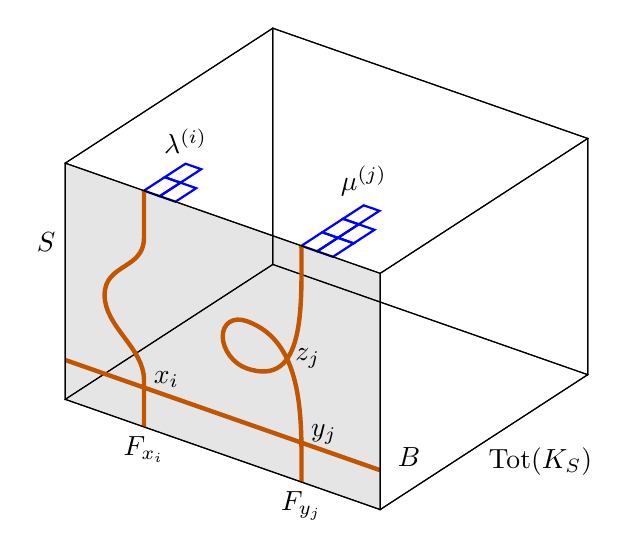
\begin{tikzpicture}[
                    %x  = {(-0.5cm,-0.5cm)},
                    %x  = {(-0.4,-1.0)},
                     %x  = {(1,-.25)},
                    %y  = {(2cm,0cm)},
                    %y  = {(0.5,1)},
                    %y  = {(0,1)},
                    %z  = {(0cm,1cm)},
                    %z  = {(1,1)},
                    %z  = {(-1,-1)},
                    z  = {-15},
		    scale = 1]
%                    scale = 0.75]

\begin{scope}[yslant=-0.35,xslant=0]
  


%\draw [ultra thick ,green , ->] (0,0,0)--node[right]{$x$ axis} (1,0,0);
%\draw [ultra thick ,blue , ->] (0,0,0)--node[right]{$y$ axis} (0,1,0);
%\draw [ultra thick ,red , ->] (0,0,0)--node[left]{$z$ axis} (0,0,1);

%left side
\begin{scope} [canvas is yz plane at x=0]
\draw [black](0,0) rectangle (3,5);
\end{scope}
%bottom side
\begin{scope} [canvas is xz plane at y=0]
\draw [black](0,0) rectangle (4,5);
\end{scope}
%back
\draw [black](0,0) rectangle (4,3);


% partitions
\begin{scope} [canvas is xz plane at y=3]
%1st partition
\draw [thick,blue](1,5) rectangle (1.2,4.5);
\draw [thick,blue](1.2,5) rectangle (1.4,4.5);
\draw [thick,blue](1,4.5) rectangle (1.2,4.0);
%\draw [thick,blue](1.2,4.5) rectangle (1.4,4.0);
%2nd partition
%\draw [thick,blue](2,5) rectangle (2.2,4.5);
%\draw [thick,blue](2.2,5) rectangle (2.4,4.5);
%\draw [thick,blue](2,4.5) rectangle (2.2,4.0);
%\draw [thick,blue](2.2,4.5) rectangle (2.4,4.0);
%3rd partition
\draw [thick,blue](3,5) rectangle (3.2,4.5);
\draw [thick,blue](3.2,5) rectangle (3.4,4.5);
\draw [thick,blue](3,4.5) rectangle (3.2,4.0);
\draw [thick,blue](3.2,4.5) rectangle (3.4,4.0);
\draw [thick,blue](3,4.0) rectangle (3.2,3.5);
\end{scope}





%smooth fiber
\draw [ultra thick,orange] 
                   (1  ,0   ,5)
to [out=90,in=-90] (1  ,0.6 ,5)
to [out=90,in=-90] (0.5,1.5 ,5)
to [out=90,in=-90] (1  ,2.4 ,5)
to [out=90,in=-90] (1  ,3   ,5);

%section

\draw [ultra thick,orange] (0,0.5,5)--(4,0.5,5);

%nodal fiber
\draw [ultra thick,orange] 
                    (3   ,0   ,5) 
to [out=90,in=0]    (2.3 ,1.8 ,5) 
to [out=180,in=90]  (2   ,1.5 ,5) 
to [out=270,in=180] (2.3 ,1.2 ,5) 
to [out=0,in=270]   (3   ,3   ,5);



\node [above] at (3,3,3.5) {$\mu^{(j)} $};
\node [below] at (3,0,5) {$F_{y_{j}}$};
\node [right] at (3,0.6,5) {$y_{j}$};
\node [right] at (2.8,1.5,5) {$z_{j}$};
\node [above] at (1,3,4) {$\lambda^{(i)}$};
\node [below] at (1,0,5) {$F_{x_{i}}$};
\node [right] at (1,0.6,5) {$x_{i}$};
\node [left] at (0,2.0,5) {$S$};
\node [right] at (4.2,0,3) {$\operatorname{Tot}(K_{S})$};
\node [right] at (4.1,0.7,5) {$B$};



%right side
\begin{scope} [canvas is yz plane at x=4]
\draw [black](0,0) rectangle (3,5);
%diagonal curve
%\draw [pink, ultra thick, domain=0:3, samples=100] 
%plot (\x ,{5*pow(sin(28.8*pi*\x),2)});
\end{scope}
%top side
\begin{scope} [canvas is xz plane at y=3]
\draw [black](0,0) rectangle (4,5);
\end{scope}
%front
\draw [black](0,0,5) rectangle (4,3,5);
\draw [black,fill, opacity=0.1](0,0,5) rectangle (4,3,5);


\end{scope}
\end{tikzpicture}
\caption{Cohen-Macaulay curve $Z_{\CM}$ with underlying reduced
support in orange and thickenings $\lambda^{(i)}$ along smooth fibers
$F_{x_{i}}$, $\mu^{(j)}$ along singular fibers $F_{y_{j}}$, and
multiplicity one along the section $B$.}\label{fig: drawing of Cohen-Macaulay C^* fixed subscheme}
\end{figure}



\begin{proposition} \label{nest}
A closed points $Z$ of $\Hilb^{d,\bullet}(X)^{\CC^*}$ correspond to a finite nesting of closed subschemes of $S$
$$
Z_{0} \supset Z_{1} \supset \cdots \supset Z_{l},
$$
satisfying
$$
\sum_{k=0}^{l} [Z_k] = B + dF \in H_2(S).
$$
\end{proposition}

\proof 
Using projection $\pi : X \rightarrow S$, a quasi-coherent sheaf on
$X$ can be viewed as a quasi-coherent sheaf $\F$ on $S$ together with
a morphism $\F \otimes K_{S}^{-1} \rightarrow \F$. A
$\CC^*$-equivariant structure on $\F$ translates into a $\ZZ$-grading
$$
\pi_* \F = \bigoplus_{k \in \ZZ} \F_k,
$$
such that $\F \otimes K_{S}^{-1} \rightarrow \F$ is graded, i.e.
$$
\F_k \otimes K_{S}^{-1} \longrightarrow \F_{k-1}.
$$
Here $\F_k$ has weight $k$ and $K_{S}$ weight $1$ under the $\CC^*$-action. The structure sheaf $\O_X$ corresponds to 
$$
\pi_* \O_X = \bigoplus_{k=0}^{\infty} K_{S}^{-k}.
$$
Therefore a $\CC^*$-equivariant morphism $\F \rightarrow \O_X$ corresponds to a graded sheaf $\F$ as above together with maps
\begin{displaymath}
\xymatrix
{
\cdots & \F_1 \ar[d] & \oplus & \F_0 \ar[d] & \oplus & \F_{-1} \ar[d] & \oplus & \F_{-2} \ar[d] & \cdots \\
\cdots &  0 & \oplus & \O_S & \oplus & K_{S}^{-1} & \oplus & K_{S}^{-2} & \cdots, 
}
\end{displaymath}
where 
\begin{displaymath}
\xymatrix
{
\F_k \otimes K_{S}^{-1} \ar[r] \ar[d] & \F_{k-1} \ar[d] \\
K_{S}^{k} \otimes K_{S}^{-1} \ar@{=}[r] & K_{S}^{k-1}
}
\end{displaymath}
commute for all $k\leq 0$ and the composition $\F_1 \otimes K_{S}^{-1} \rightarrow \F_0 \rightarrow \O_S$ is to zero. 

It is useful to re-define $\G_k := \F_{-k} \otimes K_{S}^{k}$. Then a $\CC^*$-equivariant morphism $\F \rightarrow \O_X$ is equivalent to the following data:
\begin{itemize}
\item quasi-coherent sheaves $\{\G_k\}_{k \in \ZZ}$ on $S$,
\item morphisms $\{\G_k \rightarrow \G_{k+1}\}_{k \in \ZZ}$,
\item morphisms $\G_k \rightarrow \O_S$ such that the following diagram commutes:
\end{itemize}
\begin{displaymath}
\xymatrix
{
\cdots \ar[r] & \G_{-1} \ar[d] \ar[r] & \G_0 \ar[r] \ar[d] & \G_{1} \ar[r] \ar[d] & \G_{2} \ar[r] \ar[d] & \cdots \\
\cdots \ar[r] & 0 \ar[r] & \O_S \ar@{=}[r]& \O_S \ar@{=}[r] & \O_S \ar@{=}[r] & \cdots 
}
\end{displaymath}
In the case of interest to us $\G \rightarrow \O_X$ is an ideal sheaf $I_Z \hookrightarrow \O_X$ cutting out $Z \subset X$. In the above language, this means $\G_k = 0$ for $k<0$, the morphisms $\G_k \rightarrow \O_S$ are injective, and the morphisms $\G_k \rightarrow \G_{k+1}$ are injective. Therefore $\G_k = I_{Z_k \subset S}$ is an ideal sheaf cutting out $Z_k \subset S$ and 
$$
I_{Z_k \subset S} \subset I_{Z_{k+1} \subset S},
$$
for all $k$. \qed 


Let $\Hilb^{B+dF}(S)$ be the Hilbert scheme of effective divisors on $S$ with class $$B+dF \in H_2(S).$$ By Lemma \ref{Hilbcvs} of the Appendix \ref{appHilb}, pull-back along $p$ and adding the section $B$ induces an isomorphism
$$
\Sym^d(B) \cong \Hilb^{B+dF}(S).
$$
%This allows us to see the curves on $S$. 

For any reduced curve $C \subset S$ defined by ideal sheaf $I_{C \subset S}$ and $d >0$, we denote by $dC$ the Gorenstein curve defined by the ideal sheaf $I_{C \subset S}^d$, the $d$th power of $I_{C \subset S}$. We combine Lemma \ref{Hilbcvs} with a (family version of) Proposition \ref{nest} to conclude the following:
\begin{proposition} \label{proprho}
There exists a morphism
$$
\rho_d : \Hilb^{d,n}(X)^{\CC^*} \longrightarrow \Sym^d(B), 
$$
which at the level of closed points can be can be described as follows. Let $Z \in \Hilb^{d,n}(X)^{\CC^*}$ and let $Z_{\CM} \subset Z$ be the maximal Cohen-Macaulay subcurve of $Z$. Since $Z_{\CM}$ is $\CC^*$-fixed, its ideal sheaf decomposes
$$
I_{Z_{\CM}} = \bigoplus_{k=0}^{\infty} I_{Z_k \subset S} \otimes K_{S}^{-k},
$$
where 
$$
Z_0 = B \cup \lambda_{0}^{(1)} F_{x_1} \cup \cdots \cup \lambda_{0}^{(l)} F_{x_l}
$$
for some distinct closed points $x_i \in B$ and $\lambda_{0}^{(i)} > 0$, and
$$
Z_k = \lambda_{k}^{(1)} F_{x_1} \cup \cdots \cup \lambda_{k}^{(l)} F_{x_l}.
$$
for some $\lambda_{k}^{(i)} \leq \lambda_{k-1}^{(i)}$. Here $\lambda^{(i)} = (\lambda^{(i)}_{0} \geq \lambda^{(i)}_{1} \geq \cdots)$ define 2D partitions satisfying 
$$
\sum_{i=1}^{l} |\lambda^{(i)}| = d.
$$
See Figure~\ref{fig: drawing of Cohen-Macaulay C^* fixed subscheme}
for an illustration. The map $\rho_d$ sends $Z$ to 
$$
\sum_{i=1}^{l} |\lambda^{(i)}| x_i \in \Sym^d(B).
$$
\end{proposition}

\begin{remark}
The morphism of this proposition is perhaps somewhat surprising. Since we are on a 3-fold, the map which sends a closed subscheme of $Z \in \Hilb^{d,n}(X)$ to its underlying Cohen-Macaulay curve $Z_{\CM}$ is \emph{not} a morphism. Nevertheless, the map $\rho_d$ which records the location of the fibres in $Z_{\CM}$ and their multiplicities is a morphism.
\end{remark}

\begin{proof}
The description of $\rho_d$ at the level of closed points is clear. We construct $\rho_d$ as a morphism from Proposition \ref{nest} and Lemma \ref{Hilbcvs} of Appendix \ref{appHilb}.

Let $T$ be an arbitrary base scheme of finite type and let 
$$
\Z \subset X \times T
$$
be a $\CC^*$-fixed and $T$-flat closed subscheme. Assume for each $t \in T$ the fibre $\Z_t$ has class $B+dF \in H_2(S)$ and $\chi(\O_{\Z_t}) = n$. Since $\Z$ is $\CC^*$-fixed, Proposition \ref{nest} implies that its ideal sheaf decomposes\footnote{The arguments leading to Proposition \ref{nest} hold equally well for $T$-flat families over a base $T$.}
$$
I_{\Z} = \bigoplus_{k = 0}^{\infty} I_{\Z_k \subset S \times T} \otimes K_{S}^{-k},
$$
where $K_{S}$ is pulled-back along $S \times T \rightarrow S$ and 
$$
\Z_0 \supset \Z_1 \supset \cdots.
$$
Then each $\Z_k \subset S \times T$ is $T$-flat as well. The maximal CM subschemes $\Z_{k, \CM} \subset \Z_k \subset S \times T$ are also $T$-flat \todo{I can provide explanation why $\Z_{\CM,k}$ also $T$-flat. Needed?} and induces morphisms
\begin{align*}
T &\longrightarrow \Hilb^{B + d_0 F}(S), \\ 
T &\longrightarrow \Hilb^{d_k F}(S),  \textrm{ \ for \ } k>0
\end{align*}
where $\sum_k d_k = d$. Adding divisors gives a morphism $T \longrightarrow \Hilb^{B+dF}(S)$. By Lemma \ref{Hilbcvs}, we obtain a morphism $T \rightarrow \Sym^d(B)$. This morphism corresponds to a $T$-flat family for $\Sym^d(B)$. We have defined $\rho_d$ as a morphism. 
\end{proof}

%In the above proposition, each $Z_k \subset S$ contains a maximal Cohen-Macaulay (in fact, Gorenstein) subcurve $D_k$ such that $Z_k \setminus D_k$ is 0-dimensional. For $k=0$, $D_0$ is the scheme-theoretic union of the section $B$ and thickenings of certain distinct fibres $F_{x_1}$, $\ldots$, $F_{x_n}$. Denoting the orders of thickenings by $\lambda_{0}^{(1)}, \ldots, \lambda_{0}^{(n)} > 0$, we obtain\footnote{For any reduced curve $C$ on a surface $S$ with ideal sheaf $I_C \subset \O_S$ and $d>0$, we denote by $d C$ the scheme defined by the ideal sheaf $I_{C}^{d} \subset \O_S$.}
%$$
%D_0 = B \cup \lambda_{0}^{(1)} F_{x_1} \cup \cdots \cup \lambda_{0}^{(n)} F_{x_n}.
%$$
%This statement follows from Corollary \ref{cor: chow(beta) = sym (B)} of the appendix. Next, for all $i = 1, \ldots, n$ and $k \geq 1$, there are $\lambda_{k}^{(i)} \leq \lambda_{k-1}^{(i)}$ such that
%$$
%D_k = \lambda_{k}^{(1)} F_{x_1} \cup \cdots \cup \lambda_{k}^{(n)} F_{x_n}.
%$$
%We conclude:
%\begin{proposition} \label{ZCM}
%To each closed point $Z$ of $\Hilb^{d,\bullet}(X)^{\CC^*}$ correspond distinct closed points $x_1, \ldots, x_n \in B$ for some $n$ and (finite) 2D partitions $\lambda^{(1)}, \ldots, \lambda^{(n)}$ such that
%$$
%\sum_{i=1}^{n} |\lambda^{(i)}| = d.
%$$
%The maximal Cohen-Macaulay subcurve of $Z$ is given by the scheme-theoretic union of the zero section $B$ and the schemes with ideal sheaves
%$$
%\bigoplus_{k=0}^{\infty} \O_{S}(-\lambda_{k}^{(i)} F_{x_i}) \otimes K_{S}^{-k},
%$$
%for all $i = 1, \ldots, n$.
%\end{proposition}

%Note that in the notation of this proposition, the morphism $\rho_d$ in \eqref{rho} maps $Z$ to
%$$
%\sum_{i=1}^{n} |\lambda^{(i)}| x_i \in \Sym^d(B),
%$$
%where $|\lambda^{(i)}|$ denotes the size of the 2D partition $\lambda^{(i)}$.
%This leads to the following proposition:
%\begin{proposition} \label{C^*}
%For each $h>0$, there exists a stratification
%$$
%\Hilb^{h,\bullet}(X)^{\CC^*} = \coprod_{n=1}^{\infty} \coprod_{{\scriptsize{\begin{array}{c} \lambda^{(1)}, \ldots, \lambda^{(n)} \mathrm{s.t.} \\ \sum_{\alpha=1}^{n} |\lambda^{(\alpha)}| = h \end{array}}}} \Hilb^{h,\bullet}_{\lambda^{(1)}, \ldots, \lambda^{(n)}}(X)^{\CC^*},
%$$
%where $\Hilb^{h,\bullet}_{\lambda^{(1)}, \ldots, \lambda^{(n)}}(X)^{\CC^*}$ is the locally closed subset of subschemes $Z \subset X$ with maximal Cohen-Macaulay curve defined by the scheme-theoretic union of $B$ and schemes with ideal sheaves of the form \eqref{CMcurve} for some distinct fibre $F_{x_1}, \ldots, F_{x_n} \subset S$.
%\end{proposition}

%In this proposition, the number of points $n$ and the position of the points $x_1, \ldots, x_n \in B$ can still vary freely. We now want to refine the stratification by fixing the position of these points.


\section{Push-forward to the symmetric product} \label{sym}

In the previous section we constructed a morphism (Proposition \ref{proprho}) 
\begin{equation} \label{rho}
\rho_{d} : \Hilb^{d,\bullet}(X)^{\CC^*} \longrightarrow \Sym^d(B).
\end{equation}
We obtain
$$
\int_{\Hilb^{d,\bullet}(X)^{\CC^*}} 1 \, de = \int_{\Sym^d(B)} \rho_{d*}(1) \, de,
$$
where $f_d:= \rho_{d*}(1)$ is the $\ZZ ((p))$-valued constructible function on
$\Sym^d(B)$ given by pushing forward the Euler characteristic
measure. \todo{JB: Do we know a reference for this fact about integrals
with respect to euler char measure and pushforwards? I think it is
simply the fact that pushforward (in the sense of taking euler char of
fibers of a function) is constructible. MK: The reference is Prop.~1 of MacPherson's ``Chern classes for singular algebraic varieties''. Do we add this?} Its value at a closed point
$\mathfrak{a} \in \Sym^d(B)$ is
$$
f_d(\mathfrak{a}) = \int_{\rho_{d}^{-1}(\mathfrak{a})} 1 \, de.
$$
We are interested in the calculation of
$$
\DThat (X) = \sum_{d \geq 0} q^d \int_{\Sym^d(B)} f_d \, de.
$$
It turns out that the constructible function $f_d : \Sym^d(B) \rightarrow \ZZ(\!(p)\!)$ satisfies two multiplicative properties. The first one is described as follows. Denote by $B^{\sm} \subset B$ the open subset over which the fibres are smooth and by $B^{\sing}$ the $N$ points over which the fibres are singular. We can consider the restrictions of $f_d$ to $\Sym^d(B^{\sm}) \subset \Sym^d(B)$ and $\Sym^d(B^{\sing}) \subset \Sym^d(B)$. Denote by $M(p)$ the MacMahon function.
\begin{proposition} \label{mult1}
Let $d_1, d_2 \geq 0$ be such that $d_1+d_2 = d$. Then 
%there are constructible functions
%\begin{align*}
%g_{d_1} : \Sym^{d_1}(B^{\sm}) &\longrightarrow \ZZ(\!(p)\!) \\
%h_{d_2} : \Sym^{d_2}(B^{\sing}) &\longrightarrow \ZZ(\!(p)\!),
%\end{align*}
%such that for any $\sum_i a_i x_i \in \Sym^{d_1}(B^{\sm})$ and $\sum_j b_j y_j \in \Sym^{d_2}(B^{\sing})$ \todo{Forgot: points which can are off the curve.}
$$ 
f_d(\mathfrak{a} + \mathfrak{b}) =\frac{(p^{\frac{1}{2}} - p^{-\frac{1}{2}})^{e(B)}}{M(p)^{e(X)}} \cdot f_{d_1}(\mathfrak{a}) \cdot f_{d_2}(\mathfrak{b}), 
$$
for any $\mathfrak{a} \in \Sym^{d_1}(B^{\sm})$ and $\mathfrak{b} \in \Sym^{d_2}(B^{\sing})$. 
\end{proposition}
We prove this proposition in Section \ref{chargh}. The following product formula is an immediate consequence of this result
\begin{align}
\begin{split} \label{firstprod}
%&\sum_{d \geq 0} q^d \int_{\Sym^d(B)} f_d \, de = \\
\DThat (X)  = \frac{(p^{\frac{1}{2}} - p^{-\frac{1}{2}})^{e(B)}}{M(p)^{e(X)}}  \Bigg( \sum_{d \geq 0} q^d \int_{\Sym^d(B^{\sm})} f_d \, de \Bigg) \cdot \Bigg( \sum_{d \geq 0} q^d \int_{\Sym^d(B^{\sing})} f_d \, de \Bigg). 
\end{split}
\end{align}
The restricted constructible functions $f_d  : \Sym^d(B^{\sm}) \rightarrow \ZZ(\!(p)\!)$ and $f_d  : \Sym^d(B^{\sing}) \rightarrow \ZZ(\!(p)\!)$ satisfy further multiplicative properties:
\begin{proposition} \label{mult2}
There exist functions $g : \ZZ_{\geq 0} \rightarrow \ZZ(\!(p)\!)$ and $h : \ZZ_{\geq 0} \rightarrow \ZZ(\!(p)\!)$ taking values in formal Laurent series $\ZZ(\!(p)\!)$, such that $g(0)=1$, $h(0)=1$, and
\begin{align*}
f_{d}(\mathfrak{a}) &= \frac{M(p)^{e(X)}}{(p^{\frac{1}{2}} - p^{-\frac{1}{2}})^{e(B)}} \cdot \prod_{i=1}^l g(a_i), \\
f_{d}(\mathfrak{b}) &= \frac{M(p)^{e(X)}}{(p^{\frac{1}{2}} - p^{-\frac{1}{2}})^{e(B)}} \cdot \prod_{j=1}^m h(b_j), 
\end{align*}
for all $\mathfrak{a} = \sum_{i=1}^l a_i x_i \in \Sym^{d}(B^{\sm})$, and $\mathfrak{b} = \sum_{j=1}^m b_j y_j \in \Sym^{d}(B^{\sing})$, where $x_i \in B^{\sm}$ and $y_j \in B^{\sing}$ are collections of distinct closed points.
\end{proposition}
We prove this proposition in Section \ref{chargh}. Together with Lemma \ref{lem: formula for euler char of sym products} of Appendix \ref{power}, Proposition \ref{mult2} and equation \eqref{firstprod} imply
\begin{equation} \label{initialprod}
%\sum_{d \geq 0} q^d \int_{\Sym^d(B)} f_d \, de 
\DThat (X) = \frac{M(p)^{N}}{(p^{\frac{1}{2}} - p^{-\frac{1}{2}})^{e(B)}} \cdot \Bigg( \sum_{a=0}^{\infty} g(a) q^a \Bigg)^{e(B) - N} \cdot \Bigg( \sum_{b=0}^{\infty} h(b) q^b \Bigg)^N.
\end{equation}
Our goal is to prove Propositions \ref{mult1} and \ref{mult2}, and find formulae for $g(a)$, $h(b)$. This requires a better understanding of the strata
$$
\rho_{d}^{-1} (\mathfrak{a} + \mathfrak{b}) \subset \Hilb^{d, \bullet}(X)^{\CC^*},
$$
for all $\mathfrak{a} \in \Sym^{d_1}(B^{\sm})$ and $\mathfrak{b} \in \Sym^{d_2}(B^{\sing})$ with $d_1+d_2=d$. Suppose 
\begin{align*}
\mathfrak{a} &= \sum_{i=1}^{l} a_i x_i \in \Sym^{d_1}(B^{\sm}), \\
\mathfrak{b} &= \sum_{j=1}^{m} b_j y_j \in \Sym^{d_2}(B^{\sing}),
\end{align*}
where  $x_i \in B^{\sm}$ and $y_j \in B^{\sing}$ are collections of distinct closed points. Proposition \ref{proprho} gives a decomposition of $\rho_{d}^{-1} ( \mathfrak{a} + \mathfrak{b} )$ into components\footnote{We use the term component somewhat loose: it means a subset which is both open and closed. We do not care whether it is connected.}
\begin{equation} \label{comps}
\bigsqcup_{{\scriptsize{\begin{array}{c} \lambda^{(1)} \vdash a_1 \\ \cdots \\ \lambda^{(l)} \vdash a_l \end{array}}}} \bigsqcup_{\scriptsize{\begin{array}{c} \mu^{(1)} \vdash b_1 \\ \cdots \\ \mu^{(m)} \vdash b_m \end{array}}} \Sigma(x_1, \ldots, x_l, y_1, \ldots, y_m, \lambda^{(1)}, \ldots, \lambda^{(l)}, \mu^{(1)}, \ldots, \mu^{(m)}).
\end{equation}
We abbreviate these components by $\Sigma(\boldsymbol{x};\boldsymbol{y};\boldsymbol{\lambda};\boldsymbol{\mu})$. Therefore $\Sigma(\boldsymbol{x};\boldsymbol{y};\boldsymbol{\lambda};\boldsymbol{\mu})$ is the stratum of points $Z \in \Hilb^{d,\bullet}(X)^{\CC^*}$, for which the maximal Cohen-Macaulay subcurve $Z_{\CM} \subset Z$ is determined by the data $\boldsymbol{x}, \boldsymbol{y}, \boldsymbol{\lambda}, \boldsymbol{\mu}$ as in Proposition \ref{proprho}. Note that these strata have a natural scheme structure: the fibres of $\rho_d$ are closed subschemes of $\Hilb^{d,\bullet}(X)^{\CC^*}$ and these strata are components of them. We are interested in the Euler characteristics of these strata. In the next section, we will see that the Euler characteristic of $\Sigma(\boldsymbol{x};\boldsymbol{y};\boldsymbol{\lambda};\boldsymbol{\mu})$ does \emph{not} depend on the exact location of the points $x_i \in B^{\sm}$ and $y_j \in B^{\sing}$, but only on their number $m$ and $n$ and the partitions $\lambda^{(i)}$ and $\mu^{(j)}$.


\section{Restriction to formal neighbourhoods} \label{formal}

In the previous two sections we reduced our consideration to the strata $\Sigma(\boldsymbol{x};\boldsymbol{y};\boldsymbol{\lambda};\boldsymbol{\mu})$ of $Z \in \Hilb^{d,\bullet}(X)^{\CC^*}$ for which the maximal Cohen-Macaulay subcurve $Z_{\CM} \subset Z$ is determined by the data $\boldsymbol{x}, \boldsymbol{y}, \boldsymbol{\lambda}, \boldsymbol{\mu}$. In this section we break down this stratum further by cutting it up in pieces covered by formal neighbourhoods. For notational simplicity, we first consider the case where the base point is 
$$
a x + b y \in \Sym^d(B),
$$
with $x \in B^{\sm}$, $y \in B^{\sing}$, and $d=a+b$. We show how to compute $e(\Sigma(x,y,\lambda,\mu))$. Once this case is established, it is not hard to generalize to arbitrary $e(\Sigma(\boldsymbol{x};\boldsymbol{y};\boldsymbol{\lambda};\boldsymbol{\mu}))$. This leads to a proof of Propositions \ref{mult1} and \ref{mult2}, and a geometric characterization of the functions $g(a)$, $h(b)$ of Section \ref{sym}.


\subsection{Fpqc cover}

The idea is to use an appropriate cover of $X$ and calculate on pieces of the cover. We first give a complex analytic definition of the cover to aid the intuition and then give the actual ``algebro-geometric cover'': 
\begin{enumerate}
\item The reduced support $B \cup F_x \cup F_y$ has three singular points\footnote{Recall that $x,y \in B$ in the base can be viewed as points on $S$ and $X$ via the sections $B \subset S \subset X$.}: $x,y \in B$ and $z \in F^{\sing}_{y}$. We take small open balls around these points.
\item Consider the punctured curve $B^\circ := B \setminus \{x,y\}$ and let $X^\circ := X \setminus (F_x  \cup F_y)$. We take a tubular neighbourhood of $B^\circ \subset X^\circ$.
\item Consider the punctured curve $F_{x}^{\circ} := F_x \setminus \{x\}$ and let $X^\circ := X \setminus B$. We take a tubular neighbourhood of $F_{x}^\circ \subset X^\circ$.
\item Consider the punctured curve $F_{y}^{\circ} := F_y \setminus \{y,z\}$ and let $X^\circ := X \setminus (B \cup \{z\})$. We take a tubular neighbourhood of $F_{y}^{\circ} \subset X^\circ$.
\item Finally, we take $W = X \setminus (B \cup F_x \cup F_y)$. 
\end{enumerate}

In order to work in algebraic geometry, in (1) we take the formal neighbourhood $\Xhat _x$ of $\{x\}$ in $X$. Denote the local ring at $x$ by $(R,\mathfrak{m})$. By $\Xhat _x$ we mean the (non-noetherian) scheme
$$
\Spec \varprojlim R / \mathfrak{m}^n 
$$
and \emph{not} the formal scheme $$\mathrm{Spf} \varprojlim R / \mathfrak{m}^n.$$ Similarly in (2) and (3), let $\Xhat _y$ be the formal neighbourhood of $\{y\}$ in $X$ and $\Xhat _z$ the formal neighbourhood of $\{z\}$ in $X$. Note that 
$$
\Xhat _x \cong \Xhat _y \cong \Xhat _z \cong\Spec \CC[\![x_1,x_2,x_3]\!].
$$
Even though $\Xhat _x$ is non-noetherian, the morphism $\Xhat _x \rightarrow X$ has a good property: it is fpqc so can be used as part of a cover \cite[Sect.~2.3.2]{Vis}. Flatness of this map follows from the fact that formal completion is an exact operation \cite[Prop.~10.14]{AM}.\todo{Completion is faithfully flat: stacks project Lem.~10.96.3.} 

In (2) we consider $B^\circ := B \setminus \{x,y\}$, $X^\circ := X \setminus (F_x  \cup F_y)$ and let $\Xhat ^{\circ}_{B^\circ}$ be the formal neighbourhood of $F_{x}^{\circ}$ in $X^\circ$. For (3) and (4) the formal neighbourhoods $\Xhat ^{\circ}_{F_{x}^{\circ}}$ and $\Xhat ^{\circ}_{F_{y}^{\circ}}$ are defined analogously. Note that the definition of $X^\circ$ in (2)--(4) varies. Finally in (5) we take $W = X \setminus (B \cup F_x \cup F_y)$. Then
$$
\mathfrak{U} = \{\Xhat _x \rightarrow X, \Xhat _y \rightarrow X, \Xhat _z \rightarrow X, \Xhat ^{\circ}_{B^\circ} \rightarrow X, \Xhat ^{\circ}_{F_{x}^{\circ}} \rightarrow X, \Xhat ^{\circ}_{F_{y}^{\circ}} \rightarrow X, W \subset X\}
$$
is an fpqc cover of $X$. Consequently the data of a quasi-coherent sheaf on $X$ is equivalent to the data of quasi-coherent sheaves on each of the opens of $\mathfrak{U}$ and gluing isomorphisms between the restrictions on the overlaps. Technically: quasi-coherent sheaves on $X$ form a stack with respect to the fpqc topology \cite[Thm.~4.23]{Vis}.


\subsection{Local moduli spaces} \label{localmod}

We now introduce moduli spaces of closed subschemes of dimension $\leq 1$ on the pieces of the cover $\mathfrak{U}$. Assume the coordinates on $$\Xhat _x \cong \Spec \CC[\![ x_1,x_2,x_3]\!]$$ are chosen such that $x_1=x_3=0$ corresponds to the intersection $\Xhat _x \times_X B$ and $x_2=x_3=0$ corresponds to $\Xhat _x \times_X F_x$. Define
\begin{align*}
&\Hilb^{(1,d),n}(\Xhat _x) := \\
&\big\{ I_Z \subset \O_{\Xhat _x} \ : \ [Z] = [\Xhat _x \times_X B] + d [\Xhat _x \times_X F_x] \ {\rm{and}} \ h^0(I_{Z_{\CM}} / I_Z) = n \big\}.
\end{align*}
Here the equation
$$
[Z] = [\Xhat _x \times_X B] + d [\Xhat _x \times_X F_x]
$$
means $Z$ is supported along $$(\Xhat _x \times_X B) \cup (\Xhat _x \times_X F_x)$$ with multiplicity 1 along $\Xhat _x \times_X B$ and multiplicity $d$ along $\Xhat _x \times_X F_x$ and $Z_{\CM}$ denotes the maximal Cohen-Macaulay subcurve of $Z$. The ideal sheaves fit into a short exact sequence
$$
0 \longrightarrow I_{Z} \longrightarrow I_{Z_{\CM}} \longrightarrow Q \longrightarrow 0, 
$$
where $Q$ is 0-dimensional. The Hilbert scheme $\Hilb^{(1,d),n}(\Xhat _y)$ is defined likewise replacing the point $x$ by $y$. For $\Xhat _z$, we define
$$
\Hilb^{d,n}(\Xhat _z) := \big\{ I_Z \subset \O_{\Xhat _z} \ : \ [Z] = d [\Xhat _z \times_X F_y] \ {\rm{and}} \ h^0(I_{Z_{\CM}} / I_Z) = n \big\}.
$$
Each of $\Xhat _x, \Xhat _y, \Xhat _z$ has an action of $\CC^*$ compatible with the fibre scaling on $X$. This action lifts to the moduli space. Since each of these formal neighbourhoods is isomorphic to $\Spec \CC[\![x_1,x_2,x_3]\!]$, the bigger torus $\CC^{*3}$ acts on it and this action lifts to the moduli space. The existence of these ``extra actions'' will be used in Section \ref{vertex}.

Next consider $\Xhat ^{\circ}_{B^\circ}$, i.e.~the formal neighbourhood of the punctured zero section $B^\circ \subset X^\circ$. Define
$$
\Hilb^{1,n}(\Xhat ^{\circ}_{B^\circ}) := \big\{ I_Z \subset \O_{\Xhat ^{\circ}_{B^\circ}} \ : \ [Z] = [\Xhat ^{\circ}_{B^\circ} \times_X B] \ {\rm{and}} \ h^0(I_{Z_{\CM}} / I_Z) = n \big\}.
$$
For $\Xhat ^{\circ}_{F_{x}^{\circ}}$, $\Xhat ^{\circ}_{F_{y}^{\circ}}$ we define
\begin{align*}
\Hilb^{d,n}(\Xhat ^{\circ}_{F_{x}^{\circ}}) &:= \big\{ I_Z \subset \O_{\Xhat ^{\circ}_{F_{x}^{\circ}}} \ : \ [Z] = d [\widehat{F}_{x}^{\circ}] \ {\rm{and}} \ h^0(I_{Z_{\CM}} / I_Z) = n \big\}, \\
\Hilb^{d,n}(\Xhat ^{\circ}_{F_{y}^{\circ}}) &:= \big\{ I_Z \subset \O_{\Xhat ^{\circ}_{F_{y}^{\circ}}} \ : \ [Z] = d [\widehat{F}_{y}^{\circ}] \ {\rm{and}} \ h^0(I_{Z_{\CM}} / I_Z) = n \big\}.
\end{align*}
Finally for $W$ we define
$$
\Hilb^{0,n}(W) := \big\{ I_Z \subset \O_{W} \ : \ \dim(Z) = 0 \ {\rm{and}} \ h^0(\O_Z) = n \big\}.
$$
On $\Xhat ^{\circ}_{B^\circ}$, $\Xhat ^{\circ}_{F_{x}^{\circ}}$, $\Xhat ^{\circ}_{F_{y}^{\circ}}$, and $W$ we have an action of $\CC^*$ compatible with the fibre scaling on $X$. These actions lift to the moduli space. However, \emph{unlike} for $\Xhat _x$, $\Xhat _y$, $\Xhat _z$, no additional tori act.

As before, we use the notation $\Hilb^{(1,d),\bullet}(\Xhat _x)$ for the union of all $\Hilb^{(1,d),n}(\Xhat _x)$ and similarly for all other moduli spaces of this section. Like in Section \ref{fixedlocus}, the components of the $\CC^*$-fixed locus of $\Hilb^{(1,d),\bullet}(\Xhat _x)$ are indexed by 2D partitions 
$$
\Hilb^{(1,d),\bullet}(\Xhat _x)^{\CC^*} = \bigsqcup_{\lambda \vdash d} \Hilb^{(1,d),\bullet}(\Xhat _x)_{\lambda}^{\CC^*}.
$$

\begin{proposition} \label{bij}
Consider the stratum $\Sigma(x,y,\lambda,\mu)$, where $|\lambda|=a$ and $|\mu|=b$. Restriction from $X$ to the elements of the cover $\mathfrak{U}$ induces a morphism
\begin{align}
\begin{split} \label{restr}
\Sigma(x,y,\lambda,\mu) \longrightarrow &\Hilb^{(1,a),\bullet}(\Xhat _x)_{\lambda}^{\CC^*} \times \Hilb^{(1,b),\bullet}(\Xhat _y)_{\mu}^{\CC^*} \times \Hilb^{b,\bullet}(\Xhat _z)_{\mu}^{\CC^*} \times \\
&\Hilb^{1,\bullet}(\Xhat ^{\circ}_{B^\circ})^{\CC^*} \times \Hilb^{a,\bullet}(\Xhat ^{\circ}_{F_{x}^{\circ}})_{\lambda}^{\CC^*} \times \Hilb^{b,\bullet}(\Xhat ^{\circ}_{F_{y}^{\circ}})_{\mu}^{\CC^*} \times \\
&\Hilb^{0,\bullet}(W)^{\CC^*},
\end{split}
\end{align}
which is a bijection on closed points.
\end{proposition}
\begin{proof}
Since pull-back works in families, restriction indeed defines a morphism. For the rest of the proof, we work on closed points only.

Since $\mathfrak{U}$ is an fpqc cover, fpqc descent implies that any ideal sheaf $I_Z \subset \O_X$ is entirely determined by its restriction along the morphisms of the elements of $\mathfrak{U}$. This proves injectivity.

Conversely, given local ideal sheaves in the image of \eqref{restr},
their restrictions to overlaps only depend on the underlying
Cohen-Macaulay curve and not on the embedded points. Since we chose
the strata such that the underlying Cohen-Macaulay curve is already
fixed, there are no further gluing conditions and fpqc descent implies
surjectivity.
\end{proof}
   
\begin{remark}
Note that the argument of Proposition \ref{bij} produces a bijective
morphism --- we do \emph{not} claim \eqref{restr} is an
isomorphism of schemes. However, a bijective morphism induces an
equality of (topological) Euler characteristic, which is what we use.
\end{remark}

\begin{remark}
It is important to relate holomorphic Euler characteristic of domain and target in \eqref{restr}. For any subscheme $Z$ in the domain $\Sigma(x,y,\lambda,\mu)$, denote the corresponding maximal Cohen-Macaulay curve of its elements by $Z_{\CM}$ (Proposition \ref{proprho}). Then
$$
\chi(\O_Z) = \chi(\O_{Z_{\CM}}) + \chi(I_{Z_{\CM}} / I_{Z}).
$$ 
Recall that $Z_{\CM}$ is entirely determined by the data $x,y, \lambda, \mu$, where $\lambda = (\lambda_0 \geq \lambda_1 \geq \cdots)$ and $\mu = (\mu_0 \geq \mu_1 \geq \cdots)$ are 2D partitions (equation \eqref{comps}). An easy calculation shows 
$$
\chi(\O_{Z_{\CM}}) = \chi(\O_B) - \lambda_0 - \mu_0.
$$
We conclude
\begin{equation} \label{relchi}
\chi(\O_Z) = \frac{e(B)}{2} - \lambda_0 - \mu_0 + \chi(I_{Z_{\CM}} / I_{Z}).
\end{equation}
\end{remark}

Proposition \ref{bij} allows us to calculate 
$$
f_d(ax+by) = e(\rho_{d}^{-1}(ax+by)) = \sum_{\lambda \vdash a} \sum_{\mu \vdash b} e(\Sigma(x,y,\lambda,\mu)).
$$
By Proposition \ref{bij} and \eqref{relchi} 
\begin{align}
\begin{split} \label{fdintermediate}
f_d(ax+by) = \ &p^{\frac{e(B)}{2}} e(\Hilb^{1,\bullet}(\Xhat ^{\circ}_{B^{\circ}})^{\CC^*}) \, e(\Hilb^{0,\bullet}(W)^{\CC^*}) \times \\
&\sum_{\lambda \vdash a} \sum_{\mu \vdash b} p^{- \lambda_0 - \mu_0 } e(\Hilb^{(1,a),\bullet}(\Xhat _{x})_{\lambda}^{\CC^*}) \, e(\Hilb^{(1,b),\bullet}(\Xhat _{y})_{\mu}^{\CC^*}) \times \\
&e(\Hilb^{b,\bullet}(\Xhat _{z})_{\mu}^{\CC^*}) \, e(\Hilb^{a,\bullet}(\Xhat ^{\circ}_{F_{x}^{\circ}})_{\lambda}^{\CC^*}) \, e(\Hilb^{b,\bullet}(\Xhat ^{\circ}_{F_{y}^{\circ}})_{\mu}^{\CC^*}).
\end{split}
\end{align}

Before we proceed, we calculate $e(\Hilb^{0,\bullet}(W)^{\CC^*})$ and $e(\Hilb^{1,\bullet}(\Xhat ^{\circ}_{B^{\circ}})^{\CC^*})$. The first follows from a formula of J.~Cheah \cite{Che} 
\begin{equation} \label{Cheah}
e(\Hilb^{0,\bullet}(W)^{\CC^*}) = M(p)^{e(W)}.
\end{equation}
For the second we use the following proposition:
\begin{proposition} \label{section}
Let $x_1, \ldots, x_l \in B$ be any number of distinct closed points. Define 
\begin{align*}
B^\circ &:= B \setminus \{x_1, \ldots, x_l\}, \\
X^\circ &:= X \setminus \bigsqcup_{i=1}^{l} F_{x_i}.
\end{align*} 
Let $\Xhat ^{\circ}_{B^{\circ}}$ be the formal neighbourhood of $B^\circ$ in $X^\circ$. Define $\Hilb^{1,n}(\Xhat ^{\circ}_{B^{\circ}})$ to be the Hilbert scheme of subschemes $Z \subset \Xhat ^{\circ}_{B^{\circ}}$, such that $Z_{\CM} = B^\circ$ and $\chi(I_{Z_{\CM}} / I_Z) = n$.
%, where $Z_{CM}$ denotes the maximal Cohen-Macaulay subscheme contained in $Z$ (Proposition \ref{ZCM}). 
Then
$$
e(\Hilb^{1,\bullet}(\Xhat ^{\circ}_{B^{\circ}})) = \Bigg( \frac{M(p)}{1-p} \Bigg)^{e(B^\circ)}.
$$
\end{proposition}
\begin{proof}
Pick any $y \in B^\circ$ and let $\Xhat _{y} \cong \Spec \CC [\![x_1,x_2,x_3]\!]$ be the formal neighbourhood of $y$ in $X^\circ$. Denote by $$\Hilb^{1,n}(\Xhat ^{\circ}_{y})$$ the Hilbert scheme of subschemes $Z \subset \Xhat _{y}^{\circ}$, such that $Z_{\CM} = \{x_1=x_3=0\}$ and $\chi(I_{Z_{\CM}} / I_Z) = n$. 

We have projections
$$
X^\circ \longrightarrow S^\circ \longrightarrow B^\circ.
$$
These map induces a morphism
$$
\Hilb^{1,n}(\Xhat ^{\circ}_{B^{\circ}}) \longrightarrow \Sym^n(B^\circ).
$$
The fibre over a point $\mathfrak{a} = \sum_i a_i y_i$, with all $y_i \in B^\circ$ distinct, equals
$$
\prod_{i} \Hilb^{1,a_i}(\Xhat _{y_i}^{\circ}).
$$
%This follows by using an appropriate fpqc cover of $B^\circ$ similar to Proposition \ref{bij}. 
Since $B$ is reduced and smooth, $\Hilb^{1,a_i}(\Xhat _{y_i}^{\circ})$ only depends on $a_i$ and not on the point $y_i \in B^\circ$. Therefore Lemma \ref{lem: formula for euler char of sym products} of Appendix \ref{power} implies
$$
e(\Hilb^{1,\bullet}(\Xhat ^{\circ}_{B^{\circ}})) = \Bigg( \sum_{a=0}^{\infty} e(\Hilb^{1,a}(\Xhat _{y}^{\circ})) p^a \Bigg)^{e(B^\circ)}.
$$
The formal neighbourhood $\Xhat _{y}$ has an action of $\CC^{*3}$ and this action lifts to $\Hilb^{1,a}(\Xhat _{y})$. The fixed locus consists of a finite number of points counted by the topological vertex\footnote{Discussed in general in Section \ref{vertex}.}
\begin{equation*}
\sfV_{\square\varnothing\varnothing} = \frac{M(p)}{1-p}. \qedhere
\end{equation*}
%The proof follows.
\end{proof}

Using \eqref{fdintermediate}, \eqref{Cheah}, and Proposition \ref{section} gives
\begin{align*}
f_d(ax+by) = \ &\frac{M(p)^{e(X)}}{(p^{\frac{1}{2}}-p^{-\frac{1}{2}})^{e(B)}} \times \\
&(1-p) \sum_{\lambda \vdash a} p^{-\lambda_0} e(\Hilb^{(1,a),\bullet}(\Xhat _x)_{\lambda}^{\CC^*}) \, e(\Hilb^{a,\bullet}(\Xhat ^{\circ}_{F_{x}^{\circ}})_{\lambda}^{\CC^*}) \times \\
&\frac{1-p}{M(p)} \sum_{\mu \vdash b} p^{-\mu_0} e(\Hilb^{(1,b),\bullet}(\Xhat _y)_{\mu}^{\CC^*}) \, e(\Hilb^{b,\bullet}(\Xhat _z)_{\mu}^{\CC^*}) \, e(\Hilb^{b,\bullet}(\Xhat ^{\circ}_{F_{y}^{\circ}})_{\mu}^{\CC^*}).
\end{align*}

   
\subsection{Geometric characterization of $g(a)$ and $h(b)$} \label{chargh}

The arguments of the preceding two sections are straightforwardly modified to any stratum $\Sigma(\boldsymbol{x};\boldsymbol{y};\boldsymbol{\lambda};\boldsymbol{\mu})$. Fix a smooth fibre $F_x$ and a singular fibre $F_y$. Denote the singular point of $F_y$ by $z$. Let $\Xhat _x$, $\Xhat _z$ be the formal neighbourhoods of $x$, $z$ in $X$. Define $\Hilb^{(1,a),\bullet}(\Xhat _x)$, $\Hilb^{b,\bullet}(\Xhat _z)$ as in Section \ref{localmod}. Like in Section \ref{localmod}, we also consider the ``tubular'' formal neighbourhoods $\Xhat ^{\circ}_{F_{x}^{\circ}}$, $\Xhat ^{\circ}_{F_{y}^{\circ}}$ and corresponding Hilbert schemes $\Hilb^{a,\bullet}(\Xhat ^{\circ}_{F_{x}^{\circ}})$, $\Hilb^{b,\bullet}(\Xhat ^{\circ}_{F_{y}^{\circ}})$. A straightforward generalization of the calculation of $f_d(ax+by) $ yields:
\begin{proposition} \label{geomgh}
For any $a,b>0$ define
\begin{align*}
g(a) &:= (1-p) \sum_{\lambda \vdash a} p^{-\lambda_0} e(\Hilb^{(1,a),\bullet}(\Xhat _x)_{\lambda}^{\CC^*}) \, e(\Hilb^{a,\bullet}(\Xhat ^{\circ}_{F_{x}^{\circ}})_{\lambda}^{\CC^*}), \\
h(b) &:= \frac{1-p}{M(p)} \sum_{\mu \vdash b} p^{-\mu_0} e(\Hilb^{(1,b),\bullet}(\Xhat _y)_{\mu}^{\CC^*}) \, e(\Hilb^{b,\bullet}(\Xhat _z)_{\mu}^{\CC^*}) \, e(\Hilb^{b,\bullet}(\Xhat ^{\circ}_{F_{y}^{\circ}})_{\mu}^{\CC^*}),
\end{align*}
and let $g(0) := 1$, $h(0) :=1$. Then
\begin{align*}
f_{d}(\mathfrak{a} + \mathfrak{b}) &= \frac{M(p)^{e(X)}}{(p^{\frac{1}{2}}-p^{-\frac{1}{2}})^{e(B)}} \cdot \prod_{i} g(a_i) \cdot \prod_{j} h(b_j), 
\end{align*}
for any $\mathfrak{a} = \sum_i a_i x_i \in \Sym^{d}(B^{\sm})$ and $\mathfrak{b} = \sum_j b_j y_j \in \Sym^{d}(B^{\sing})$, where $x_i \in B^{\sm}$ and $y_j \in B^{\sing}$ are collections of distinct closed points.
\end{proposition}
   
We immediately deduce:  
\begin{corollary} 
Propositions \ref{mult1} and \ref{mult2} are true for $g(a)$ and $h(b)$ defined in Proposition \ref{geomgh}.
\end{corollary}   
   
   
\section{Reduction to the topological vertex}  \label{vertex} 

In this section, we obtain (Theorem~\ref{thm: Zhat in terms of
vertex}) expressions for $\DThat (X)$ and $\DThat_{\fiber }(X)$ in
terms of the topological vertex $\sfV_{\lambda\mu\nu}(p)$, $e(B)$, and
$N$ (the number of nodal fibres). The theorem follows by expressing
$g(a)$ and $h(b)$ of Proposition \ref{geomgh} in terms of the
topological vertex.


\subsection{Point contributions}   

Following the conventions of \cite{BKY}, we denote by 
$$
\sfV_{\lambda\mu\nu} = \sum_{\pi} p^{|\pi|}, 
$$
the topological vertex. Here the sum is over all 3D partitions $\pi$
with outgoing legs $\lambda, \mu, \nu$ and $|\pi|$ denotes
renormalized volume (see Definitions (1) and (2) in \cite{BKY}). For a
2D partition $\lambda = (\lambda_0 \geq \lambda_1 \geq \cdots)$, we
write $\lambda'$ for the corresponding transposed partition and
\begin{align*}
|\lambda| &:= \sum_{k=0}^{\infty} \lambda_k, \\
|\!|\lambda|\!|^2 &:= \sum_{k=0}^{\infty} \lambda_{k}^{2}.
\end{align*}

\begin{proposition} \label{vertex1}
Let $F_x$ be a smooth fibre and $F_y$ a singular fibre with singularity $z$. Then for any $\lambda \vdash a$, $\mu \vdash b$
\begin{align*}
p^{-\lambda_0} e(\Hilb^{(1,a),\bullet}(\Xhat _x)_{\lambda}^{\CC^*}) &= \sfV_{\lambda\square\varnothing}, \\
p^{-\mu_0} e(\Hilb^{(1,b),\bullet}(\Xhat _y)_{\mu}^{\CC^*}) &= \sfV_{\mu\square\varnothing}, \\
p^{-|\!|\mu|\!|^2} e(\Hilb^{b,\bullet}(\Xhat _z)_{\mu}^{\CC^*}) &= \sfV_{\mu\mu'\varnothing}.
\end{align*}
\end{proposition}
\begin{proof}
Recall that $$\Xhat _x \cong \Xhat _y \cong \Xhat _z \cong \Spec \CC[\![x_1,x_2,x_3]\!].$$ Therefore, $\CC^{*3}$ acts on each of these schemes and their moduli spaces 
$$
\Hilb^{(1,a),\bullet}(\Xhat _x)_{\lambda}^{\CC^*}, \ \Hilb^{(1,b),\bullet}(\Xhat _y)_{\mu}^{\CC^*}, \ \Hilb^{b,\bullet}(\Xhat _z)_{\mu}^{\CC^*}.
$$
The coordinates can be chosen such that the action of the last factor
of $\CC^{*3}$ corresponds to $x_3 \mapsto t_3 x_3$. This component
acts trivially since we are already on the $\CC^*$-fixed locus. The
$\CC^{*3}$-fixed locus consists of isolated reduced points
corresponding to monomial ideals with asymptotics
$(\lambda,\varnothing,\varnothing)$, $(\mu,\varnothing,\varnothing)$,
$(\mu,\mu',\varnothing)$ respectively\footnote{The transpose in $\mu'$
occurs, because we follow the orientation convention of
\cite{BKY}.}. These monomial ideals are exactly what the topological
vertex counts.

Finally, note that the generating functions
$e(\Hilb^{(1,a),\bullet}(\Xhat _x)_{\lambda}^{\CC^*})$,
$e(\Hilb^{(1,b),\bullet}(\Xhat _y)_{\mu}^{\CC^*})$,
$e(\Hilb^{b,\bullet}(\Xhat _z)_{\mu}^{\CC^*})$ all start with $1$. On
the other hand, from the definition
\begin{align*}
\sfV_{\lambda\square\varnothing} &= p^{-\lambda_0} + \cdots, \\
\sfV_{\mu\square\varnothing} &= p^{-\mu_0} + \cdots, \\
\sfV_{\mu\mu'\varnothing} &= p^{-\sum_{k=0}^{\infty} \mu_{k}^{2}} + \cdots,
\end{align*}
where $\cdots$ stands for higher order terms in $p$. The proposition follows.
\end{proof}


\subsection{Fibre contribution}

Let $F_x$ be a smooth fibre and $F_y$ a singular fibre. Recall the
formal neighbourhoods $\Xhat ^{\circ}_{F_{x}^{\circ}}$, $\Xhat
^{\circ}_{F_{y}^{\circ}}$ of Section \ref{formal}.
\begin{proposition} \label{vertex2}
For any $\lambda \vdash a$ and $\mu \vdash b$, we have
\begin{align*}
e(\Hilb^{a,\bullet}(\Xhat ^{\circ}_{F_{x}^{\circ}})_{\lambda}^{\CC^*}) &= \frac{1}{\sfV_{\lambda\varnothing\varnothing}}, \\
e(\Hilb^{b,\bullet}(\Xhat ^{\circ}_{F_{y}^{\circ}})_{\mu}^{\CC^*}) &= \frac{1}{\sfV_{\mu\varnothing\varnothing}}.
\end{align*}
\end{proposition}
\begin{proof}
********
\end{proof}   


\subsection{Putting it together.}

Combining Proposition \ref{geomgh} with Propositions \ref{vertex1}, \ref{vertex2} gives:
\begin{proposition} \label{combgh}
For any $a,b>0$ 
\begin{align}
\begin{split} \label{gh}
g(a) &= (1-p) \sum_{\lambda \vdash a} \frac{\sfV_{\lambda\square\varnothing}}{\sfV_{\lambda\varnothing\varnothing}}, \\
h(b) &= \frac{1-p}{M(p)} \sum_{\mu \vdash b} p^{|\!|\mu|\!|^2} \frac{\sfV_{\mu\square\varnothing}}{\sfV_{\mu\varnothing\varnothing}} \sfV_{\mu\mu'\varnothing}.
\end{split}
\end{align}
\end{proposition}

Putting all our results together, we obtain formulas for the partition
functions in terms of the vertex: 
\begin{theorem} \label{thm: Zhat in terms of vertex}
\begin{align*}
\DThat (X)& = \frac{1}{(p^{\frac{1}{2}} - p^{-\frac{1}{2}})^{e(B)}} \Bigg( (1-p) \sum_{\lambda} q^{|\lambda|} \frac{\sfV_{\lambda\square\varnothing}}{\sfV_{\lambda\varnothing\varnothing}} \Bigg)^{e(B) - N}  \Bigg( (1-p) \sum_{\mu}  q^{|\mu|} p^{|\!|\mu|\!|^2} \frac{\sfV_{\mu\square\varnothing}}{\sfV_{\mu\varnothing\varnothing}} \sfV_{\mu\mu'\varnothing} \Bigg)^{N} \\
\DThat_{\fiber}(X)&= \Bigg( \sum_{\lambda} q^{|\lambda|} \Bigg)^{e(B) - N} \Bigg( \sum_{\mu} q^{|\mu|} p^{|\!|\mu|\!|^2} \sfV_{\mu\mu'\varnothing} \Bigg)^{N}.
\end{align*}
\end{theorem}
\begin{proof}
Inserting the equations for $g(a)$, $h(b)$ of Proposition \ref{combgh}
into \eqref{initialprod} gives the formula for $\DThat (X)$. Similar
reasoning\dots \todo{Go back and put in the necessary stuff so that
the $\DThat_{\fiber}$ computation isn't just hand waving.}
\end{proof}

\begin{corollary}
Theorem~\ref{thm: main thm -- formulas for DT and DTfiber} is true.
\end{corollary}
\begin{proof}
We apply the main theorem of \cite{BKY}. In particular, we substitute
\cite[Eqns~(2)\&(4)]{BKY} into the formula for $\DThat (X)$ and we substitute
\cite[Eqn~(1)]{BKY}, as well as the well-known formula
\[
\sum_{\lambda}q^{|\lambda |} =\prod_{d=1}^{\infty}\frac{1}{(1-q^{d})}
\]
into the formula for $\DThat_{\fiber } (X)$.
\end{proof}

\section{Putting in the Behrend function} \label{sec: Behrend}

The aim of this section is to show that the partition functions
$\DThat (X)$ and $\DT (X)$ are equal after the simple change of
variables $y=-p$. In order to do this we will need to assume a
conjecture about the Behrend function which we formulate below for
general Calabi-Yau threefolds.

Let $Y$ be any quasi-projective Calabi-Yau
threefold.  Let $C\subset Y$ be a (not necessarily reduced)
Cohen-Macaulay curve with proper support. Assume that the
singularities of $C_{\red}$ are locally toric\footnote{This means that
formally locally $C_{\red}$ is either smooth, nodal, or the union of
the three coordinate axes. That is at $p\in C_{\red}\subset Y$ the
ideal $\widehat{I}_{C_{\red}}\subset \widehat{\mathcal{O}}_{Y,p}$ is
given by $(x_{1},x_{2})$, $(x_{1},x_{2}x_{3})$, or
$(x_{1}x_{2},x_{2}x_{3},x_{1}x_{3})$ for some isomorphism
$\widehat{\mathcal{O}}_{Y,p}\cong \CC
[[x_{1},x_{2},x_{3}]]$. }. Define\emph{
\[
\Hilb^{C,n}(Y) = \{Z\subset Y \text{ such that $C\subset Z$ and
$I_{C}/I_{Z}$ has finite length $n$} \}.
\]
}
Note that $\Hilb^{C,n}(Y)\subset \Hilb (Y)$ and let $\nu$ denote the
Behrend function on $\Hilb (Y)$. Our conjecture is the following:

\begin{conjecture}\label{conj: Behrend fnc conj}
\[
\int_{\Hilb^{C,n}(Y)} \nu \, de = (-1)^{n} \nu ([C]) \int_{\Hilb^{C,n}(Y)} \, de
\]
where $\nu ([C])$ is the value of the Behrend function at the point $[C]\in \Hilb (Y)$.
\end{conjecture}

\begin{remark}
Conceivably, the condition that $C_{\red}$ has locally toric
singularities could be weakened, although we do not have any evidence
for this case. Our conjecture is true for $Y$ a (globally) toric
Calabi-Yau. This follows from the computations in \cite{MNOP1}.

One could also make the much stronger conjecture that 
\[
\nu ([Z]) = (-1)^{n} \nu ([C])
\]
for all $[Z]\in \Hilb^{C,n}(Y)$. This would of course imply our
conjecture as stated. However, we do not know if this stronger version
holds, even in the case where $Y$ is $\CC^{3}$ and $C$ is empty. In
this case, this stronger conjecture says that the Behrend function
on $\Hilb^{n}(\CC^{3})$ is the constant function $(-1)^{n}$.
\end{remark}



\appendix
\section{Odds and Ends}\label{appendix: odds and ends}

\subsection{Curves on elliptic surfaces}\label{appHilb}

Let $p : S \rightarrow B$ be an elliptic surface with section $B \subset S$. In this appendix we allow any type of singular fibres. We assume $S$ is not a product, which implies
$$
p^* : \Pic^0(B) \stackrel{\cong}{\longrightarrow} \Pic^0(S)
$$
is an isomorphism \cite[VII.1.1]{Mir}. For any $\beta \in H_2(S)$, we denote by $\Hilb^\beta(S)$ the Hilbert scheme of effective divisors on $S$ in class $\beta$. 

Denote by $B \in H_2(S)$ the class of the section $B \subset S$ and by $F \in H_2(S)$ the class of the fibre. Then we have the following commutative diagram 
\begin{displaymath}
\xymatrix
{
\Sym^d(B) \ar[d]^{p^*} \ar[r] & \Pic^d(B) \ar[d]^{p^*}_{\cong} \\
\Hilb^{dF}(S) \ar[d]^{+B} \ar[r] & \Pic^{dF}(S) \ar[d]^{\otimes \O_S(B)}_{\cong} \\
\Hilb^{B+dF}(S) \ar[r] & \Pic^{B+dF}(S). 
}
\end{displaymath}
The horizontal arrows are Abel-Jacobi maps. The vertical arrows are induced by pull-back and adding the section $B \subset S$. 
%The following is the main result of this appendix:
\begin{lemma} \label{Hilbcvs}
The above maps induce an isomorphism
$$
\Sym^d(B) \stackrel{\cong}{\longrightarrow} \Hilb^{B+dF}(S).
$$
\end{lemma}

%\begin{remark}
%The upshot of this proposition is that we can now \emph{see} the elements of $\Hilb^{B+dF}(S)$ lying in our surface $S$.
%\end{remark}

\begin{proof}
Clearly $p^*$ gives an isomorphism $\Sym^d(B) \cong \Hilb^{dF}(S)$ and $+B$ defines a closed embedding $\Hilb^{dF}(S) \hookrightarrow \Hilb^{B+dF}(S)$. Since $\Sym^d(B)$ is smooth and $\Hilb^{B+dF}(S)$ is reduced (by \cite[Lect.~25]{Mum}), it suffices to show  
$$
\Sym^d(B) \rightarrow \Hilb^{B+dF}(S)
$$ 
is surjective on closed points.

For surjectivity, suppose $D'$ is an effective divisor with class $B+dF$ which does \emph{not} lie in the image. Firstly, we note that for any fibre $F$ we have $D' \cdot F = 1$. Therefore $D'$ contains a section $B' \subset S$ as an effective summand. Moreover $B \neq B'$ or else $D'$ would lie in the image. Next, we take any $D$ in the image and compare $D$ and $D'$. Then 
$$
\O_S(D-D') \in \Pic^0(S) \cong \Pic^0(B).
$$ 
Therefore after re-arranging we find that there are distinct fibres $F_{x_i}$, $F_{y_j}$ and $a_i \geq 0$, $b_j \geq 0$ such that 
$$
B + \sum_i a_i F_{x_i} \sim_{\mathrm{lin}} B' + \sum_j b_j F_{y_j},
$$
where $\sim_{\mathrm{lin}}$ denotes linear equivalence. Hence there exists a pencil $\{C_t \}_{t \in \PP^1}$ of effective divisors such that
$$
C_0 = B + \sum_i a_i F_{x_i}, \ C_{\infty} = B' + \sum_j b_j F_{y_j}.
$$
Now fix a smooth fibre $F$. Then $C_t \cdot F = 1$ for any $t \in \PP^1$, so we get a morphism
$$
\PP^1 \longrightarrow F, \ t \mapsto C_t \cap F.
$$
But $F$ is a smooth elliptic curve so this map is constant. We conclude
$$
B \cap F = C_0 \cap F = C_{\infty} \cap F = B' \cap F.
$$
Since $F$ was chosen arbitrary, we deduce that $B = B'$ which is a contradiction.
\end{proof}

%Proof with additional assumption $d > 2g-2$:
%Since $d > 2g-2$ the Abel-Jacobi map 
%$$
%\Sym^d(B) \rightarrow \Pic^d(B)
%$$
%is a projective bundle with fibres linear systems of dimension $d-g$. We immediately deduce that all horizontal arrows of the commutative diagram are surjective. At the level of fibres, we have inclusions of linear systems
%\begin{equation} \label{epsilon}
%|\epsilon| \hookrightarrow |p^* \epsilon| \hookrightarrow |p^* \epsilon (B)|,
%\end{equation}
%where $\epsilon \in \Pic^d(B)$. We want to prove that all these linear systems have the same dimension (Claim). The first map is clearly an isomorphism since
%$$
%H^0(S,p^* \epsilon) \cong H^0(B, \epsilon \otimes p_* \O_S) = H^0(B,\epsilon)
%$$
%where we used the projection formula and $p_* \O_S \cong \O_B$. Surjectivity of the second map of \eqref{epsilon} requires more work and is proved below. Before we prove Claim, we show it implies the proposition. Choose Poincar\'e line bundles 
%\begin{align*}
%\cP &\textrm{ \ on \ } \Pic^d(B) \times B, \\
%\cQ &\textrm{ \ on \ } \Pic^{dF}(S) \times S, \\
%\cR &\textrm{ \ on \ } \Pic^{B+dF}(S) \times S.
%\end{align*}
%In each case, denote projection to the base Picard by $\pi_{\Pic}$. Since $d > 2g-2$, the sheaf $\pi_* \mathcal{P}$ is locally free because the dimensions of $|\epsilon|$, $\epsilon \in \Pic^d(B)$ do not jump. Using the isomorphism $\Pic^d(B) \cong \Pic^{dF}(S)$, we see that pull-back of $\mathcal{P}$ along 
%$$
%\Pic^{dF}(S) \times S \rightarrow \Pic^d(B) \times B
%$$
%equals $\mathcal{Q}$ (up to tensoring by a line bundle pulled-back from $S$, which we get rid of by redefining $\mathcal{Q}$). We write this as $p^* \mathcal{P} \cong \mathcal{Q}$. Pushing down to $\Pic^{dF}(S)$, using the projection formula and $p_* \O_S \cong \O_B$, we obtain
%$$
%\pi_{\Pic *} \cP \cong \pi_{\Pic *} \cQ
%$$
%on $\Pic^{dF}(S) \cong \Pic^{d}(B)$. On $\Pic^{dF}(S) \times S$ we can form $\cQ(B)$ by pulling back $\O_S(B)$ along projection to the second factor. Then
%$$
%\cR \cong \cQ(B),
%$$
%on $\Pic^{B+dF}(S) \times S \cong \Pic^{dF}(S) \times S$ (again, after possibly redefining $\cR$). Multiplying by the section defining $B$ and pushing down gives a morphism
%\begin{equation} \label{vbmap}
%\pi_{\Pic *} \cQ \hookrightarrow (\pi_{\Pic *} \cQ)(B) \cong \pi_{\Pic *} \cR.
%\end{equation}
%Claim implies that the dimension of the fibres of $|p^* \epsilon(B)|$, $\epsilon \in \Pic^d(B)$ do not jump. Therefore $(\pi_{\Pic *} \cQ)(B) \cong \pi_{\Pic *} \cR$ is locally free. Since \eqref{vbmap} is a morphism of locally free sheaves, it suffices to check we have induced isomorphisms on the fibres. This is exactly the content of Claim. We conclude all Abel-Jacobi maps are projective bundles 
%\begin{align*}
%\PP(\pi_{\Pic *} \mathcal{P}) &\rightarrow \Pic^d(B), \\
%\PP(\pi_{\Pic *} \mathcal{Q}) &\rightarrow \Pic^{dF}(S), \\
%\PP(\pi_{\Pic *} \mathcal{R}) &\rightarrow \Pic^{B+dF}(S).
%\end{align*}
%and 
%$$
%\PP(\pi_{\Pic *} \mathcal{P}) \cong \PP(\pi_{\Pic *} \mathcal{Q}) \cong \PP\big((\pi_{\Pic *} \mathcal{Q})(B)\big) \cong \PP(\pi_{\Pic *} \mathcal{R}).
%$$

%What is left is the Claim: the second map of \eqref{epsilon} is an isomorphism for all $\epsilon \in \Pic^d(C)$. For any line bundle $\delta$ on $B$, the Leray spectral sequence yields the following short exact sequence
%\[
%0\to H^{1} (B,\delta ) \stackrel{\alpha}{\longrightarrow} H^{1} (S,p^{*}\delta ) \longrightarrow H^{0} (B,\delta \otimes R^{1}p _{*}\O_S ) \to 0.
%\]
%Therefore, if
%\begin{equation} \label{ineq}
%\deg( \delta) - \deg (R^1 p_* \O_S)^\vee < 0,
%\end{equation}
%then $\alpha$ is an isomorphism. Assume this is the case. The long exact cohomology sequence associated to 
%\[
%0\to p^{*}\delta (-B)\to p^{*}\delta \to \O _{B}\otimes p^{*}\delta \to 0
%\]
%is
%\[
%\dotsb \to H^{1} (S,p ^{*} \delta )\rt{\alpha }H^{1} (B,\delta )\to H^{2} (S,p ^{*}\delta (-B))\to H^{2} (S,p ^{*}\delta )\to 0,
%\]
%and since $\alpha $ is a surjection, we get an isomorphism of the last
%two terms. We apply Serre duality to that isomorphism and we use the
%fact that $K_{S} = p ^{*} (K_{B}\otimes L)$ where $L = \left(R^1 p
%_{*}\O _{S} \right)^{\vee }$ \cite[Thm.~12.1]{BPV} to obtain
%\begin{equation} \label{SDiso}
%H^{0} (S,p ^{*} (\delta ^{-1}\otimes K_{B}\otimes L) (B)) \cong H^{0}(S,p ^{*} (\delta ^{-1}\otimes K_{B}\otimes L)).
%\end{equation}
%Let $\epsilon \in \Pic^d(B)$ and take
%$$
%\delta =K_{B}\otimes L\otimes \epsilon ^{-1}.
%$$
%Then $\delta$ satisfies \eqref{ineq} if and only if $d>2g-2$, which we assumed. The lemma follows from \eqref{SDiso}.

%Jim's original:
%In this subsection we prove the following lemma and corollary, which will tell us what is the reduced support of all curves in the class $\beta =B+dF$.

%\begin{lemma}\label{lem: H0 (pi* (D) (B))=H0 (pi* (D))}
%For any line bundle $\epsilon $ on $B$, multiplication by the
%canonical section of $\O_S (B)$ induces an isomorphism
%\[
%H^{0} (S,p^{*} (\epsilon ) (B)) \cong H^{0} (S,p^{*} (\epsilon )).
%\]
%\end{lemma}

%\begin{corollary} \label{cor: chow(beta) = sym (B)}
%Let $\beta = B+dF \in H_{2} (S)$. Then the Chow variety of curves in
%the class $\beta $ is isomorphic to $\Sym ^{d} (B)$ where a point
%$\sum _{i}d_{i} x_{i}\in \Sym ^{d} (B)$ corresponds to the curve
%$B+\sum _{i}d_{i} F_{x_{i}}$.
%\end{corollary}

%\begin{proof}
%The corollary follows immediately from the lemma since the Chow
%variety is the space of effective divisors and the lemma implies that
%any effective divisor in the class $\beta $ is a union of the section
%$B$ with an effective divisor pulled back from the base.

%To prove Lemma~\ref{lem: H0 (pi* (D) (B))=H0 (pi* (D))} we proceed as
%follows. For any line bundle $\delta $ on $B$, the Leray spectral
%sequence yields the short exact sequence:\todo{I think arrows Leray go other way around. Anyway... last two terms iso when $2g-2<d$.}
%\[
%0\to H^{0} (B,\delta \otimes R^{1}p _{*}\O_S )\to H^{1} (S,p^{*}\delta )\Rt{\alpha } H^{1} (B,\delta )\to 0,
%\]
%in particular, $\alpha $ is a surjection.

%Then the long exact cohomology sequence associated to 
%\[
%0\to p^{*}\delta \otimes \O_S (-B)\to p^{*}\delta \to \O _{B}\otimes p^{*}\delta \to 0
%\]
%is
%\[
%\dotsb \to H^{1} (S,p ^{*} \delta )\rt{\alpha }H^{1} (B,\delta )\to H^{2} (S,p ^{*}\delta \otimes \O_S (-B))\to H^{2} (S,p ^{*}\delta )\to 0,
%\]
%and since $\alpha $ is a surjection, we get an isomorphism of the last
%two terms. We apply Serre duality to that isomorphism and we use the
%fact that $K_{S} = p ^{*} (K_{B}\otimes L)$ where $L = \left(R^1 p
%_{*}\O _{S} \right)^{\vee }$ \cite[Thm.~12.1]{BPV} to obtain
%\[
%H^{0} (S,p ^{*} (\delta ^{-1}\otimes K_{B}\otimes L) (B)) \cong H^{0}(S,p ^{*} (\delta ^{-1}\otimes K_{B}\otimes L)).
%\]
%Letting $\delta =K_{B}\otimes L\otimes \epsilon ^{-1}$, the lemma is
%proved. 
%\end{proof}

\subsection{Weighted Euler characteristics of symmetric products} \label{power}

In this section we prove the following formula for the weighted Euler
characteristic of symmetric products.

\begin{lemma}\label{lem: formula for euler char of sym products}
Let $B$ be a scheme of finite type over $\CC $ and let $e (B)$ be its
topological Euler characteristic. Let $g:\ZZ _{\geq 0}\to \ZZ (\!(p)\!)$
be any function with $g (0)=1$. Let $f_{d}:\Sym ^{d} (B)\to \ZZ (\!(p)\!)$
be the constructible function defined by $$f_{d} (\mathfrak{a})=\prod _{i}g (a_{i}),$$ for all $\mathfrak{a} = \sum_{i}
a_{i}x_{i} \in \Sym^d(B)$ where $x_i \in B$ are distinct closed points. Then
\[
\sum _{d=0}^{\infty } q^{d} \int _{\Sym ^{d} (B)} f_{d} \, de =
\left(\sum _{a=0}^{\infty }g (a) q^{a} \right)^{e (B)}.
\]
\end{lemma}

\begin{remark} \label{MacD}
In the special case where $g=f_{d}\equiv  1$, the lemma recovers
MacDonald's formula: $$\sum _{d=0}^{\infty }e (\Sym ^{d} (B)) \, q^{d} =
\frac{1}{(1-q)^{e (B)}}.$$ 

The lemma is essentially a consequence of the existence of a power
structure on the Grothendieck group of varieties definited by
symmetric products and the compatibility of the Euler characteristic
homomorphism with that power structure \todo{Ref? Bryan-Young?} \cite{}. For convenience's
sake, we provide a direct proof here.
\end{remark}
\begin{proof}
The $d$th symmetric product admits a stratification with strata
labelled by partitions of $d$. Associated to any partition of $d$ is a
unique tuple $(m_{1},m_{2},\dots )$ of non-negative integers with
$\sum _{j=1}^{\infty }j m_{j}=d$. The stratum labelled by
$(m_{1},m_{2},\dots )$ parameterizes collections of points where there
are $m_{j}$ points of multiplicity $j$. The full stratification is
given by:
\[
\Sym ^{d} (B) = \bigsqcup_{\begin{smallmatrix} (m_{1},m_{2},\dots )\\
\sum _{j=1}^{\infty }j m_{j}=d  \end{smallmatrix}} \left\{\left(\prod _{j=1}^{\infty }B^{m_{j}} \right) -\Delta  \right\}/ \prod _{j=1}^{\infty }\sigma _{m_{j}} 
\]
where by convention, $B^{0}$ is a point, $\Delta $ is the large
diagonal, and $\sigma _{m}$ is the $m$th symmetric group. Note that
the function $f_{d}$ is constant on each stratum and has value $\prod
_{j=1}^{\infty }g (j)^{m_{j}}$. Note also that the action of $\prod
_{j=1}^{\infty }\sigma _{m_{j}}$ on each stratum is free. 

For schemes over $\CC $, topological Euler characteristic is additive
under stratification and multiplicative under maps which are
(topological) fibrations. Thus
\[
\int _{\Sym ^{d} (B)} f_{d}\,\, de = \sum _{\begin{smallmatrix}(m_{1},m_{2},\dots )\\
\sum _{j=1}^{\infty }j m_{j}=d   \end{smallmatrix}} \left(\prod _{j=1}^{\infty } g (j)^{m_{j}} \right) \frac{e (B^{\sum _{j}m_{j}}-\Delta )}{m_{1}!\, m_{2}!\, m_{3}!\dots }.
\]

For any natural number $N$, the projection $B^{N}-\Delta \to
B^{N-1}-\Delta $ has fibers of the form $B-\{N-1\text{ points}
\}$. The fibers have constant Euler characteristic given by $e (B)-
(N-1)$ and consequently, $e (B^{N}-\Delta )= (e (B)- (N-1))\cdot e
(B^{N-1}-\Delta )$. Thus by induction, we find $e (B^{N}-\Delta ) = e
(B)\cdot (e (B)-1)\cdots (e (B)- (N-1))$ and so 
\[
\frac{e (B^{\sum _{j}m_{j}}-\Delta )}{m_{1}!\,m_{2}!\,m_{3}!\cdots } = \binom{e (B)}{m_{1},m_{2},m_{3},\cdots }
\]
where the right hand side is the generalized multinomial coefficient.

Putting it together and applying the generalized multinomial theorem,
we find
\begin{align*}
\sum _{d=0}^{\infty } q^d \int _{\Sym ^{d} (B)}f_{d}\,\,de & = \sum _{(m_{1},m_{2},\dots )} \prod _{j=1}^{\infty } \left(g (j) q^{j} \right)^{m_{j}} \binom{e (B)}{m_{1},m_{2},m_{3},\dots }\\
&=\left(1+\sum _{j=1}^{\infty }g (j) q^{j} \right)^{e (B)}
\end{align*}
which proves the lemma.   
\end{proof}

\newpage

\section{Stuff we gathered}

\subsection{Normal bundle} First order deformations of $B \subset X$ are given by $H^0(N_{B/X})$. We now calculate this. Let $\pi : X \rightarrow S$ and $p : S \rightarrow B$. Facts: (adjunction, canonical bundle of an elliptic surface)
\begin{align*}
N_{B/X} &\cong N_{B/S} \oplus K_{S}|_{B} \\
K_{B} &\cong K_{S}|_{B} \otimes N_{B/S} \cong K_{S}|_{B}(S) \\
K_S &\cong p^*(K_B \otimes L),
\end{align*}
where $L = (R^1 p_* \O_X)^{\vee}$ and 
\[
\deg L = \chi(\O_S) = \frac{e(S)}{12} = \frac{N}{12} > 0,
\]
where $N$ is the number of nodal fibres. Combining gives
\[
N_{B/S} \cong K_{B} \otimes K_{S}^{-1}|_{B} \cong L^\vee,
\] 
which has negative degree so\todo{Question: Do we not need Appendix A.1 anymore? I don't think so.} 
\[
H^0(N_{B/S}) = 0.
\]     
Next
\[
H^0(K_S|_B) \cong H^1(K_S|_{B}^{-1} \otimes K_B)^* \cong H^1(N_{B/S})^*.
\]     
By Riemann-Roch and $H^0(N_{B/S}) = 0$ we get
\[
h^1(N_{B/S}) = -\chi(N_{B/S}) = - \chi(L^\vee)= -(1-g - \chi(\O_S)) = \chi(\O_S) - 1+g.
\]     
In conclusion
\[
h^0(N_{X/B}) = \chi(\O_S) - 1+g = \frac{e(S)}{12} - \frac{e(B)}{2}.
\]     


%\subsection{Impact on Behrend function} How does this affect the overall sign of the Behrend function? The section $B$ cannot move in the surface direction and in the fibre direction we can move it by sections of 
%\[
%H^0(K_S|_B) \cong \CC^{\chi(\O_S) - 1+g}.
%\]     
%Aside: $K_{S}|_{F} = \O_F$ for each fibre $F$. Let $\Hilb^{B+\bullet F}(X)_{\CM}$ be the Hilbert scheme of \emph{naked} CM curved in class $B+\bullet F$. In the last section we hopefully see that locally formally a neighborhood of $C \in \Hilb^{B+\bullet F}(X)^{\CC^*}_{\CM}$ inside $\Hilb^{B+\bullet F}(X)_{\CM}$ is of the form\todo{I'm now being really sketchy!}
%\[
%H^0(K_S|_B) \times M,
%\]
%where $M$ is some space (which below we hopefully identify with some locus in $Y^{[n]}$ for $Y = K_{S}|_{B}$). Hence for any $C \in \Hilb^{B+\bullet F}(X)^{\CC^*}_{\CM}$ we have
%$$
%\nu(C) = (-1)^{\chi(\O_S) - 1+g} \cdot \nu_{M}(C) = (-1)^{\frac{e(S)}{12} - \frac{e(B)}{2}} \cdot \nu_{M}(C).
%$$
%Suppose $C$ is described by partitions $\lambda^{(i)}$ with
%\[
%\sum_i |\lambda^{(i)}| = d.
%\]
%We also want to prove $M$ is \emph{smooth} of dimension
%$$
%2d - \sum_i \lambda_{0}^{(i)},
%$$
%where $\lambda^{(i)} = (\lambda^{(i)}_{0} \geq \lambda^{(i)}_{1} \geq \cdots)$.\todo{Don't we also get Behrend signs $(-1)^{\lambda_{0}^{(i)}}$? Those seem bad!}


\subsection{Hilbert schemes on $\CC^2$}

Let $X = \CC^2$ and
\[
L_k := \{ Z \in X^{n} \ : \ \ell(Z \cap \{y=0\}) = k \} \subset X^{[n]}.
\]
 Claim: $L_k$ is locally closed and smooth of dimension $2n-k$. Proof: since $L_k$ is normal \todo{Why normal?} and $T = \CC^{*2}$ acts on it, it suffices to prove smoothness at $T$-fixed points\todo{Ref? I learned this from Dori Bejleri.}. At the $T$-fixed points we can write a basis for the tangent space by pairs of arrows with tail just outside and head just inside as described by Haiman. I'm not going to write this out now formally. Just remember how each arrow defines a first order deformation of the monomial ideal (``plus $\epsilon$ times the monomial the head points at''). The corresponding global deformation can easily be seen to move outside of $L_k$ for precisely $k$ arrows with head in the bottom row. This gives the result.   

\subsection{Key iso}

Let $C \in \Hilb^{B+\bullet F}(X)^{\CC^*}_{\CM}$ be described by partitions $\lambda^{(i)}$ with
\[
\sum_i |\lambda^{(i)}| = d.
\]
Claim: there is a formal neighborhood of $C$ inside $\Hilb^{B+\bullet F}(X)_{\CM}$ which maps to $H^0(N_{B/X})$ with fibre
$$
L_{k},
$$
where $k := \sum \lambda_{0}^{(i)}$ and $L_k$ is smooth by the previous subsection. 


Let's look at the case where $C = B \cup F_{\lambda}$, where $E:=F_\lambda$ is a single thickened fibre with cross-section $\lambda$. We have a couple of useful short exact sequences
\begin{align}
&0 \rightarrow I_E / I_C \rightarrow \O_C \rightarrow \O_E \rightarrow 0 \label{ses1} \\
&0 \rightarrow I_B / I_C \rightarrow \O_C \rightarrow \O_B \rightarrow 0 \label{ses2} \\
&0 \rightarrow I_C \rightarrow I_E \rightarrow I_E / I_C \rightarrow 0 \label{ses3} \\
&0 \rightarrow I_C \rightarrow I_B \rightarrow I_B / I_C \rightarrow 0, \label{ses4}
\end{align}
where 
\begin{align*}
I_E / I_C &\cong \O_B(-\lambda_0) \\
G&:=I_B / I_C,
\end{align*}
where $G$ is an ideal sheaf of a fat point of length $\lambda_0$ inside $\O_{E}$:
\begin{equation} \label{ses5}
0 \rightarrow G \rightarrow \O_E \rightarrow \O_{\lambda_0 p} \rightarrow 0.
\end{equation}
Two more significant short exact sequences
\begin{align} 
0 \rightarrow \O_C \rightarrow \O_B \oplus \O_E \rightarrow \O_{\lambda_0 p} \rightarrow 0 \label{ses6} \\
0 \rightarrow \O_B(-\lambda_0) \rightarrow \O_B \rightarrow \O_{\lambda_0 p} \rightarrow 0. \label{ses7}
\end{align}
We can build \emph{many} double complexes from these seven short exact sequences by applying $\Hom(I_C,\cdot)$, $\Hom(\cdot, \O_C)$ etc. 

It seems significant to apply $\Hom(I_E, \cdot)$ to \eqref{ses6}. This gives
\begin{equation} \label{split}
0 \rightarrow \Hom(I_E,G) \rightarrow \Hom(I_E,\O_E) \stackrel{\alpha}{\rightarrow} \Hom(I_E,\O_{\lambda_0 p}) \rightarrow \cdots
\end{equation}
The last hom space seems isomorphic to $\CC^{\lambda_0}$ and we believe there is a splitting of the map $\alpha$ from the local description. It seems $\Hom(I_E,G)$ can be interpreted as the space of deformations of $E$ which keep the length of $E \cap B$ fixed! We want to prove there exists a short exact sequence
$$
0 \rightarrow \Hom(I_E,G) \rightarrow \Hom(I_C,\O_C) \rightarrow H^0(N_{B/X}) \rightarrow 0.
$$

The good news: we can construct an injection $\Hom(I_E,G) \hookrightarrow \Hom(I_C,\O_C)$ as follows. From \eqref{ses2} and \eqref{ses3} we get the following double complex
\begin{displaymath}
\xymatrix
{
&0\ar[d]&0\ar[d]&0\ar[d]& \\
0 \ar[r] & \Hom(\O_B(-\lambda_0),G) \ar[d] \ar[r]& \Hom(\O_B(-\lambda_0),\O_C) \ar[d]\ar[r] & \Hom(\O_B(-\lambda_0),\O_B) \ar[d]\ar[r] & \cdots \\
0 \ar[r] & \Hom(I_E,G) \ar[d] \ar[r] & \Hom(I_E,\O_C) \ar[d]\ar[r] & \Hom(I_E,\O_B) \ar[d] \ar[r]& \cdots \\
0 \ar[r] & \Hom(I_C,G) \ar[d] \ar[r] & \Hom(I_C,\O_C) \ar[d] \ar[r] & \Hom(I_C,\O_B) \ar[d] \ar[r] & \cdots \\
&\cdots&\cdots&\cdots&
}
\end{displaymath}
Note: $\Hom(\O_B(-\lambda_0),G) = 0$ from the local description, so indeed we get the required injection! \\

Significant special case. When $S$ is the rational elliptic surface we have $H^0(N_{B/X}) = H^1(N_{B/X}) = 0$ in which case we get $\Hom(I_B,\O_B) = \Ext^1(I_B,\O_B) = 0$ (see next subsection for relating $\Ext^i(I_B,\O_B)$ to $H^i(N_{B/X})$)! In this case we really expect our injection
$$
\Hom(I_E,G) \hookrightarrow \Hom(I_C,\O_C)
$$
to be an isomorphism. If so, our earlier split exact sequence \eqref{split} proves $\Hom(I_C,\O_C)$ has dimension 
$$
\hom(I_E,\O_E) - \lambda_0 = \hom(I_\lambda, \O_\lambda) - \lambda_0 = 2|\lambda| - \lambda_0,
$$
where $\O_\lambda \subset \CC^{2}$ is the zero-dimensional structure sheaf from which $\O_E$ pulls-back. \\

In this special case of the rational elliptic surface we have a lot more vanishing and we hope that the big double complex yields the surjection. The easiest way to get the surjection is when
\begin{align*}
\Ext^1(G,\O_B) &\stackrel{?}{\cong} 0 \\
\Ext^1(O_B(-\lambda_0),G) &\stackrel{?}{\cong} 0,
\end{align*}
 and then use $\Hom(I_C,\O_B) \cong \Ext^1(G,\O_B)$ (which I get from $\Hom(I_B,\O_B) = \Ext^1(I_B,\O_B) = 0$). Sadly I cannot prove the two previous Ext groups are indeed zero. \\

Comment: there does not seem to be a simple map from $\Hom(I_C,\O_C) \rightarrow \Hom(I_B,\O_B)$ simply by playing with $\O_C \rightarrow \O_B$ or $I_C \subset I_B$. 


\subsection{Miscalleneous} Significant fact: $\Hom(I_C,\O_C) \cong \mathrm{Ext}^1(I_C,I_C)_0$ by PT1, Section 2.2 for naked CM curves. \\

Some remarks. By cutting out $I_B$ from a rank 2 vector bundle we get maps
\[
0 \rightarrow \Hom(I_B, \O_B) \rightarrow H^0(B,\O_B(S)) \oplus H^0(B,\O_B(Y)) \rightarrow H^0(B,\O_B(S+Y)) \rightarrow \cdots
\]
remember: $Y := K_S|_B$. Here 
\begin{align*}
\O_B(S) &\cong \O_S(S) |_{B} \cong K_X (S) |_B \cong K_S |_B \\
\O_B(Y) &\cong \O_B(B) \cong N_{B/S},
\end{align*}
and $N_{B/S} \otimes K_S|_B \cong K_B$. We get
 \[
0 \rightarrow \Hom(I_B, \O_B) \rightarrow H^0(N_{B/X}) \rightarrow H^0(K_B) \rightarrow \cdots.
\]
The first map is an isomorphism because both terms are first order deformations of $B$ as a subscheme of $X$. Not sure we need this.

\subsection{Direct approach}

We have the following commutative diagram
\begin{displaymath}
\xymatrix
{
X:=K_S \ar^{\varpi}[r] \ar_{\pi}[d] & Y:=K_S|_B \ar^{q}[d] \\
S \ar_{p}[r] & B.
}
\end{displaymath}
Note: $\pi_*$ and $q_*$ are exact (because $\pi, q$ are affine morphisms), but I don't think I need this now. I do need $\varpi^*$, $p^*$ are exact (because $\varpi, p$ are flat morphisms). Let $\Hilb^n(Y)$ be the Hilbert scheme of 0-dim subschemes of length $n$ on $Y$. By exactness of $\varpi^*$ we can pull-back
$$
0 \rightarrow I_Z \rightarrow \O_Y \rightarrow \O_Z \rightarrow 0
$$
on $Y$ to a short exact sequence
$$
0 \rightarrow \varpi^* I_Z \rightarrow \O_X \rightarrow \varpi^* \O_Z \rightarrow 0
$$
on $X$. Hence $\varpi^* \O_Z$ is a structure sheaf and $\varpi^* I_Z$ is its ideal sheaf. Let $\Hilb^0(X, [nF])$ be the Hilbert scheme of Cohen-Macaulay curves in homology class $[nF]$. Then at the set level we have a map
$$
\Hilb^n(Y) \rightarrow \Hilb^0(X,[nF]), \ (I_Z \subset \O_Y) \mapsto (\varpi^* I_Z \subset \O_X).
$$
This works in families ($(\varpi \times 1_B)^*$ is exact because $\varpi$ is flat) so this indeed gives a morphism. At the level of closed points this is clearly injective.

The tangent space at $\varpi^* I_Z \in \Hilb^0(X,[nF])$ is
\begin{align*}
\Hom_X(\varpi^* I_Z , \varpi^* \O_Z) &\cong \Hom_Y(I_Z , \varpi_* \varpi^* \O_Z) \\
&\cong \Hom_Y(I_Z , \O_Z \otimes  \varpi^* \O_X) \\
&\cong \Hom(I_Z,\O_Z),
\end{align*}
which is the tangent space at $I_Z \in \Hilb^n(Y)$. I used: (1) ordinary adjunction for $\Hom$, (2) projection formula, (3) $\varpi_* \O_X \cong \O_Y$ (how do we prove this last one? I know $\varpi_* \O_X$ is a line bundle so should go similar to $p_* \O_S \cong \O_B$). So indeed deformations match! We see there cannot be any twistings but only deformations induced from moving $Z$ in the surface. 

The next part may not be needed but I find it instructive. There is a spectral sequence
$$
\Ext^{i}_{Y}(I_Z, R^j \varpi_* \O_Z) \cong \Ext^{i}_{Y}(I_Z, \O_Z \otimes R^j \varpi_* \O_X) \Rightarrow \Ext^{i+j}_{X}(\varpi^* I_Z, \varpi^* \O_Z).
$$
Note: $R^0 \varpi_* \O_X \cong \O_Y$, $R^1 \varpi_* \O_X$ is a line bundle (the fibres of $\varpi$ have genus 1), and $R^{>1} \varpi_* \O_X = 0$ (the fibres are 1-dimensional). Therefore the terms of the spectral sequence are zero unless $j=0,1$ which leads to an injection
$$
\Ext^{1}_{Y}(I_Z,\O_Z) \hookrightarrow \Ext^{1}_{X}(\varpi^* I_Z ,\varpi^* \O_Z).
$$
This injections maps the obstruction class for deforming $Z$ to the obstruction class for deforming $\varpi^* Z$. In other words, we can deform $Z$ if and only if we can deform $\varpi^* Z$. So indeed we have an isomorphism of schemes
$$
\Hilb^n(Y) \cong \Hilb^0(X,[nF]).
$$

%\textbf{From now on it gets sketchy}... perhaps we'd like to deal with the section along the following lines... Let $\Hilb^\chi(X,[B+nF])$ be the Hilbert scheme of 1-dim subschemes with homology class $[B+nF]$ and $\chi(\O_Z) = \chi$ ($[B]$ the class of some section). We want to construct a morphism
%\begin{equation} \label{keymap}
%\Hilb^\chi(X,[B+nF]) \rightarrow H^0(N_{B/X}),
%\end{equation}
%which only remembers the section. I'm not quite sure how to do this rigorously but this sounds doable. Anyway, we want to know what $\Hilb^\chi(X,[B+nF])$ looks like near an element of the form  $B \cup C_0$, where $C_0$ is a CM curve in class $[nF]$ and $B$ a section in class $[B]$. Claim: We want to say that the scheme theoretic \emph{fibre} of \eqref{keymap} over $B \in H^0(N_{B/X})$ near $B \cup C_0$ is isomorphic to the following locally closed subset (with its induced scheme structure)
%\begin{equation} \label{locus}
%\{ C \in \Hilb^0(X,[nF]) \ : \  \chi(\O_{B \cup C}) = \chi \} \subset \Hilb^0(X,[nF]).
%\end{equation}
%The rough idea should be that by looking in the fibre of the map \eqref{keymap} we do not allow $B$ to move. Moreover an ideal sheaf of a CM curve is reflexive, hence determined entirely by its restriction to the complement of $B$. That's why the \emph{fibre} near $C_0 \cup B$ should be isomorphic to \eqref{locus}.

%Let $L_k \subset \Hilb^n(Y)$ be the locally closed subscheme of elements $Z$ such that $Z \cap B$ has length $k$. Via our isomorphism $\Hilb^n(Y) \cong \Hilb^0(X,[nF])$ the locus \eqref{locus} is clearly isomorphic to 
%$$
%L_{\chi(\O_B) - \chi},
%$$
%which is \emph{smooth}. Hence, near $B \cup C_0 \in \Hilb^\chi(X,[B+nF])$, the morphism \eqref{keymap} is a smooth morphism over a smooth base. Conclusion: near $C_0 \cup B$ we have that $\Hilb^\chi(X,[B+dF])$ is smooth (and we can calculate the dimension). I'm using the fact that a smooth morphism over a smooth base has a smooth total space.

\subsection{Koszul calculations}

Let $X = K_S$, $B \subset S \subset X$, and $Y:=K_S|_B$. For any point on $B$, I use local coordinates $x,y,z$ in a formal neighbourhood of that point such that $x=z=0$ defines the section $B$. Denote by $p : X \rightarrow Y$ the projection to $Y$. Besides the divisors $S,Y \subset X$, we have $\tilde{F} \subset X$, where $\tilde{F} = K_S|_F$ for any fibre $F \subset S$.

Let $C = B \cup p^*Z$, where $Z \subset Y$ is a 0-dimensional scheme. Assume $I_{Z \subset Y} = (z^k, y^l)$ (so the partition is a rectangle). We have the following Koszul resolution of $I_C$
\[
0 \rightarrow \O_X(-k S - l \tilde{F}) \oplus \O_X(-S - Y - l \tilde{F}) \rightarrow \O_X(-k S) \oplus \O_X(-S - l \tilde{F}) \oplus \O_X(-Y - l \tilde{F}) \rightarrow I_C \rightarrow 0,
\]
where the second map is $(z^k, y^l z, x y^l)$ and the first map is
\[
M:= \left( \begin{array}{cc} y^l & 0 \\ -z^{k-1} & x \\ 0 & -z  \end{array} \right).
\]
A local computation shows this is indeed a resolution. The second short exact sequence we use is
\[
0 \rightarrow \O_C \rightarrow \O_B \oplus \O_{p^*Z} \rightarrow \O_{P} \rightarrow 0,
\]
where $P:= B \cap p^* Z$. Using the obvious double complex, we conclude that $\Hom_X(I_C,\O_C)$ is given as the intersection of the kernels of the following two maps
\begin{align*}
\begin{array}{c} \Gamma(\O_B(kS)) \oplus \Gamma(\O_B (S+ l \tilde{F})) \oplus \Gamma(\O_B(Y \oplus l \tilde{F})) \\ \Gamma(\O_{p^*Z}(kS)) \oplus \Gamma(\O_{p^*Z} (S+ l \tilde{F})) \oplus \Gamma(\O_{p^*Z}(Y \oplus l \tilde{F})) \end{array} \stackrel{f}{\rightarrow} \begin{array}{c} \Gamma(\O_B(kS + l \tilde{F})) \oplus \Gamma(\O_B(S + l \tilde F + Y)) \\ \Gamma(\O_{p^*Z}(kS + l \tilde{F})) \oplus \Gamma(\O_{p^*Z}(S + l \tilde F + Y)) \end{array}, 
\end{align*}
and
\begin{align*}
\begin{array}{c} \Gamma(\O_B(kS)) \oplus \Gamma(\O_B (S+ l \tilde{F})) \oplus \Gamma(\O_B(Y \oplus l \tilde{F})) \\ \Gamma(\O_{p^*Z}(kS)) \oplus \Gamma(\O_{p^*Z} (S+ l \tilde{F})) \oplus \Gamma(\O_{p^*Z}(Y \oplus l \tilde{F})) \end{array} \stackrel{g}{\rightarrow} \Gamma(\O_P(kS) \oplus \Gamma(\O_P(S + l \tilde F)) \oplus \Gamma(\O_P(l \tilde F + Y)),
\end{align*}
where $f$ is given by
\[
M^T = \left( \begin{array}{ccc} y^l & -z^{k-1} & 0 \\ 0 & x & -z  \end{array} \right).
\]
and $g$ is given by taking the difference and restricting to $P$. Restricting $M^T$ to $B$ we get many zeroes and the kernel of $f$ to the part involving $B$ equals
\[
0 \oplus \Gamma(\O_B(S+l \tilde{F})) \oplus \Gamma(\O_B(Y + l \tilde{F})).
\]
The kernel of $F$ restricted to the part involving $p^*Z$ has a more complicated kernel. Certainly $\Gamma(\O_{p^*Z}(kS))$ lies in this kernel because $y^l = 0$ on $p^*Z$. Furthermore, this kernel contains all elements 
$(\beta,\gamma) \in \Gamma(p^*\O_Z(S+l\tilde{F})) \oplus \Gamma(p^*\O_Z(Y+l\tilde{F}))$ satisfying the equations
\[
-z^{k-1} \beta = 0, \ x\beta = z\gamma.
\]
This means $\beta = z \beta'$ and $\gamma = x\beta'+z^{k-1}\gamma'$. We observe that elements in the kernel of $f$ restricted to the part involving $p^*Z$ automatically restrict to zero on $P$. Therefore we should compute the kernels of 
\begin{align*}
\Gamma(\O_B(S+l \tilde{F})) &\rightarrow \Gamma(\O_P(S+l\tilde{F})) \\
\Gamma(\O_B(Y + l \tilde{F})) &\rightarrow \Gamma(\O_P(Y + l \tilde{F})),
\end{align*}
which give $\Gamma(N_{B/Y})$ and $\Gamma(N_{B/S})$! Next we should calculate the kernel of 
\[
\Gamma(\O_{p^*Z}(mS)) \rightarrow \Gamma(\O_P(mS)),
\]
which equals $\Gamma(I_{P \subset p^* Z}(mS))$. In turn this can be computed using the short exact sequence
\[
0 \rightarrow K \rightarrow I_{P \subset p^* Z} \rightarrow \O_{p^*Z}(-Y) \rightarrow 0, 
\]
where $K$ is a zero-dimensional sheaf of length $n-l$. It is not hard to see that $\Gamma(\O_{p^*Z}(mS-Y)) = 0$ so we obtain 
\[
\Gamma(I_{P \subset p^* Z}(mS)) \cong \CC^{n-l},
\]
where $n = kl$. The part which is left is $(\beta,\gamma) \in \Gamma(p^*\O_Z(S+l\tilde{F})) \oplus \Gamma(p^*\O_Z(Y+l\tilde{F}))$ satisfying
\[
\beta = z \beta', \ \gamma = x\beta'+z^{k-1}\gamma'.
\]
This is almost $\Gamma(\O_{p^*Z}(l \tilde{F}))$, which is isomorphic to $\CC^{n}$ (in which case we get $\CC^{2n-l} \oplus H^0(N_{B/Y})$ as expected!). I do not know how to account for $\gamma'$.


\begin{comment}
% Martijn's old picture:

\pgfplotsset{ticks=none}

\begin{figure}
\centering
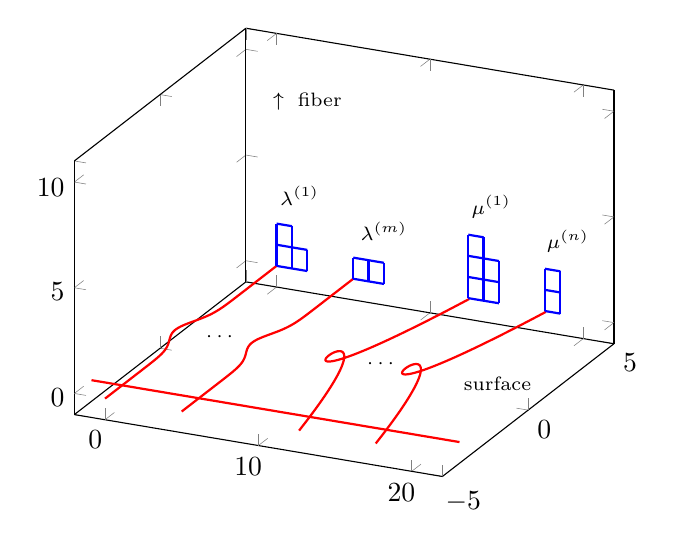
\begin{tikzpicture}
\begin{axis}
\addplot3+ [hide axis, domain=-5:5, samples=100, samples y=0,no marks, smooth,color=red,thick] ({-exp(-x^2)},{x},{0});
\addplot3+ [hide axis, domain=-5:5, samples=100, samples y=0,no marks, smooth,color=red,thick] ({-exp(-x^2)+5},{x},{0});
\addplot3+[hide axis, domain=-1.9:1.9, samples=100, samples y=0,no marks, smooth,color=red,thick] ({x^2-1+10},{x*(x^2-1)},{0});
\addplot3+[hide axis, domain=-1.9:1.9, samples=100, samples y=0,no marks, smooth,color=red,thick] ({x^2-1+15},{x*(x^2-1)},{0});
\addplot3+[hide axis, domain=-2:22, samples=100, samples y=0,no marks, smooth,color=red,thick] ({x},{-4},{0});
\addplot3 [mark=none,color=blue,thick] coordinates {(0,5,0) (2,5,0)};
\addplot3 [mark=none,color=blue,thick] coordinates {(0,5,1) (2,5,1)};
\addplot3 [mark=none,color=blue,thick] coordinates {(0,5,2) (1,5,2)};
\addplot3 [mark=none,color=blue,thick] coordinates {(0,5,0) (0,5,2)};
\addplot3 [mark=none,color=blue,thick] coordinates {(1,5,0) (1,5,2)};
\addplot3 [mark=none,color=blue,thick] coordinates {(2,5,0) (2,5,1)};
\addplot3 [mark=none,color=blue,thick] coordinates {(5,5,0) (7,5,0)};
\addplot3 [mark=none,color=blue,thick] coordinates {(5,5,1) (7,5,1)};
\addplot3 [mark=none,color=blue,thick] coordinates {(5,5,0) (5,5,1)};
\addplot3 [mark=none,color=blue,thick] coordinates {(6,5,0) (6,5,1)};
\addplot3 [mark=none,color=blue,thick] coordinates {(7,5,0) (7,5,1)};
\addplot3 [mark=none,color=blue,thick] coordinates {(12.5,5,0) (14.5,5,0)};
\addplot3 [mark=none,color=blue,thick] coordinates {(12.5,5,1) (14.5,5,1)};
\addplot3 [mark=none,color=blue,thick] coordinates {(12.5,5,2) (14.5,5,2)};
\addplot3 [mark=none,color=blue,thick] coordinates {(12.5,5,3) (13.5,5,3)};
\addplot3 [mark=none,color=blue,thick] coordinates {(12.5,5,0) (12.5,5,3)};
\addplot3 [mark=none,color=blue,thick] coordinates {(13.5,5,0) (13.5,5,3)};
\addplot3 [mark=none,color=blue,thick] coordinates {(14.5,5,0) (14.5,5,2)};
\addplot3 [mark=none,color=blue,thick] coordinates {(17.5,5,0) (18.5,5,0)};
\addplot3 [mark=none,color=blue,thick] coordinates {(17.5,5,1) (18.5,5,1)};
\addplot3 [mark=none,color=blue,thick] coordinates {(17.5,5,2) (18.5,5,2)};
\addplot3 [mark=none,color=blue,thick] coordinates {(17.5,5,0) (17.5,5,2)};
\addplot3 [mark=none,color=blue,thick] coordinates {(18.5,5,0) (18.5,5,2)};
\addplot3+ [hide axis, domain=0:10, samples=100, samples y=0,no marks, smooth,color=white,thick]    ( {-1},{1},{x});
\addplot3+ [hide axis, domain=0:0.1, samples=100, samples y=0,no marks, smooth,color=white,thick]    ( {22},{0},{x});
\node (A) at (axis cs:1.5,5,3.5) {{\scriptsize{$\lambda^{(1)}$}}};
\node (A) at (axis cs:7,5,2.5) {{\scriptsize{$\lambda^{(m)}$}}};
\node (A) at (axis cs:14,5,4.5) {{\scriptsize{$\mu^{(1)}$}}};
\node (A) at (axis cs:19,5,3.5) {{\scriptsize{$\mu^{(n)}$}}};
\node (A) at (axis cs:2,0,0) {{\scriptsize{$\cdots$}}};
\node (A) at (axis cs:12.5,0,0) {{\scriptsize{$\cdots$}}};
\node (A) at (axis cs:2,5,8) {{\scriptsize{$\uparrow \ \mathrm{fiber}$}}};
\node (A) at (axis cs:20,0,0) {{\scriptsize{$\mathrm{surface}$}}};    
\end{axis}
\end{tikzpicture}
\end{figure}
\end{comment}



\begin{comment}
% martijn's old argument for the proposition in the ``fiber
% contributions'' subsection:

We start with the first equation. Let $F := F_x \subset S$ be a smooth fibre. Consider the auxiliary surface 
$$
\tilde{S} = B \times F
$$ 
and let $Y = \mathrm{Tot}(K_{\tilde{S}})$. 
%let $e \in F$ be any closed point and consider the embeddings 
%\begin{align*}
%B &\hookrightarrow \tilde{S}, \ b \mapsto (b,e) \\
%\tilde{S} &\hookrightarrow \tilde{X}, \ p \mapsto (p,0).
%\end{align*}
Denote by $\Xhat _F$ the formal neighbourhood of $F$ in $X$ and by $\widehat{Y}_{F}$ the formal neighbourhood of
$$
F \cong \{x\} \times F \subset \tilde{S} \subset Y,
$$
where $\tilde{S} \subset Y$ denotes the zero section. In general $\Xhat _F$ and $\widehat{Y}_{F}$ are \emph{not} isomorphic. 

Denote by $\Xhat ^{\circ}_{F^\circ}$ the formal neighbourhood of $F \setminus B$ in $X \setminus B$. Recall that through the section $B \subset S$, we can view $x$ as an element of both $B$ and $F$.  We denote by $\widehat{Y}_{F^{\circ}}^{\circ}$ the formal neighbourhood of $(\{x\} \times F) \setminus (B \times \{x\})$ inside $Y \setminus (B \times \{x\})$. Since we have removed the section $B$, there exists an isomorphism \todo{Provide more argument here?} 
\begin{equation} \label{isopuncturednghs}
\Xhat ^{\circ}_{F^\circ} \cong \widehat{Y}_{F^{\circ}}^{\circ}.
\end{equation}
We are interested in the moduli space $\Hilb^{a,\bullet}(\Xhat ^{\circ}_{F^\circ})$ and the correspondingly defined moduli space $\Hilb^{a,\bullet}(\widehat{Y}^{\circ}_{F^\circ})$. Since $\Xhat ^{\circ}_{F^\circ}$ and $\widehat{Y}^{\circ}_{F^\circ}$ have (compatible) $\CC^*$-actions coming from scaling the fibres of $X$ and $Y$, we can consider their $\CC^*$-fixed loci and stratify them according to 2D partitions as in \eqref{comps}. By \eqref{isopuncturednghs}, we have an isomorphism   
$$
\Hilb^{a,\bullet}(\Xhat ^{\circ}_{F^\circ})_{\lambda}^{\CC^*} \cong \Hilb^{a,\bullet}(\widehat{Y}^{\circ}_{F^\circ})_{\lambda}^{\CC^*}.
$$
This observation allows us to work in the much simpler geometry of $Y$. This is only possible because we removed the section $B$ from $X$ and $Y$.

Let $F \cong \{x\} \times F \subset \tilde{S} \subset Y$ be as above. Denote by $\widehat{Y}_{y}$ the formal neighbourhood $y \in Y$, where $y$ is the intersection of $F \cong \{x\} \times F$ and $B \times \{x\}$ inside the zero section $\tilde{S} \subset Y$. Let $\widehat{Y}_F$, $\widehat{Y}^{\circ}_{F^\circ}$ be the formal neighbourhoods introduced above. Then we have a cover\todo{Strictly speaking: not clear these maps are flat since $\widehat{Y}_F$ non-noetherian! However: not an issue if you'd work with high enough truncation of $\widehat{Y}_F$.}
$$
\{\widehat{Y}_y \rightarrow \widehat{Y}_F, \widehat{Y}^{\circ}_{F^\circ} \rightarrow \widehat{Y}_F\}. 
$$
On these pieces, we introduce moduli spaces as in Section \ref{formal}
\begin{align*}
\Hilb^{a,\bullet}(\widehat{Y}_y), \ \Hilb^{a,\bullet}(\widehat{Y}_F), \ \Hilb^{a,\bullet}(\widehat{Y}^{\circ}_{F^\circ}).
\end{align*}
Similar to Proposition \ref{bij}, restriction gives a bijective morphism on closed points
\begin{equation} \label{bij2}
\Hilb^{a,\bullet}(\widehat{Y}_F)^{\CC^*}_{\lambda} \rightarrow \Hilb^{a,\bullet}(\widehat{Y}_y)^{\CC^*}_{\lambda} \times \Hilb^{a,\bullet}(\widehat{Y}^{\circ}_{F^\circ})^{\CC^*}_{\lambda}.
\end{equation}

Recall that $\tilde{S} = B \times F$. Then $F$ does not only act on $F \subset \tilde{S}$, but on any thickening $d F \subset \tilde{S}$. This is because
$$
\O_{dF} = \O_{d x} \otimes \O_F,
$$
where $dx \subset B$ denotes the $d$ times thickening of the point $x \in B$. Moreover, $F$ acts on the thickened curve defined by the ideal sheaf
$$
\bigoplus_{k=0}^{\infty} \O_{\tilde{S}}(-\lambda_k F) \otimes K_{\tilde{S}}^{-k}.
$$
The action of the elliptic curve $F$ on itself is fixed-point-free, so it lifts to a free action on $\Hilb^{a,\bullet}(\widehat{Y}_F)^{\CC^*}_{\lambda}$. Since $e(F) = 0$, we deduce
\begin{equation} \label{e=1}
e(\Hilb^{a,\bullet}(\widehat{Y}_F)^{\CC^*}_{\lambda}) = 1.
\end{equation}
On $\widehat{Y}_y \cong \Spec \CC[\![x_1,x_2,x_3]\!]$ we have an action of $\CC^{*3}$, so
\begin{equation} \label{001}
e(\Hilb^{a,\bullet}(\widehat{Y}_y)^{\CC^*}_{\lambda}) = e(\Hilb^{a,\bullet}(\widehat{Y}_y)^{\CC^{*3}}_{\lambda}) = \sfV_{\lambda\varnothing\varnothing}.
\end{equation}
From equations \eqref{e=1}, \eqref{bij2}, \eqref{001}, and \eqref{isopuncturednghs} we conclude that
\begin{align*}
1=e(\Hilb^{a,\bullet}(\widehat{Y}_F)^{\CC^*}_{\lambda}) &= e( \Hilb^{a,\bullet}(\widehat{Y}_y)^{\CC^*}_{\lambda}) \, e(\Hilb^{a,\bullet}(\widehat{Y}^{\circ}_{F^\circ})^{\CC^*}_{\lambda}) \\
&=  \sfV_{\lambda\varnothing\varnothing} \cdot e(\Hilb^{a,\bullet}(\widehat{Y}^{\circ}_{F^\circ})^{\CC^*}_{\lambda}) \\
&=  \sfV_{\lambda\varnothing\varnothing} \cdot e(\Hilb^{a,\bullet}(\Xhat ^{\circ}_{F^\circ})^{\CC^*}_{\lambda}).
\end{align*}

The equation for $e(\Hilb^{b,\bullet}(\Xhat ^{\circ}_{F_{y}^{\circ}})_{\mu}^{\CC^*})$ can be deduced similarly. This time, the smooth fibre $F = F_x \subset S \subset X$ is replaced by the \emph{smooth locus} of the singular fibre, i.e.~ 
$$
F' := F_{y}^{\sm} = F_{y} \setminus \{z\},
$$
where $z$ denotes the singularity of $F_y$. Note that
$$
F' \cong \PP^1 \setminus \{2 \ \rm{points}\} \cong \CC^*.
$$
Therefore, we again have a free action of $F'$ on itself and $e(F') = 0$. The rest of the proof follows the same steps.
\end{comment}

     
\begin{thebibliography}{BOPY}
\bibitem[AM]{AM} M.~F.~Atiyah and I.~G.~MacDonald, \textit{Introduction to commutative algebra}, Westview Press (1969).
%\bibitem[BCC]{BCC} J.~Bouttier, G.~Chapuy, and S.~Corteel, \textit{From Aztec diamonds to pyramids: steep tilings}, arXiv:1407.0665 [math.CO].
\bibitem[Beh]{Beh} K.~Behrend, \textit{Donaldson-Thomas type invariants via microlocal geometry}, Annals of Math.~\textbf{170} (2009), 1307--1338.
%\bibitem[BGK]{BGK} J.~Bryan, F.~Greer, and M.~Kool, \emph{in preparation}.
\bibitem[BKY]{BKY} J.~Bryan, M.~Kool, and B.~Young, \textit{Trace identities for the topological vertex}, in preparation.
%\bibitem[BO]{BO} S.~Bloch and A.Okounkov, \textit{The character of the infinite wedge representation}, Adv.~Math.~\textbf{149} (2000), 1--60.
\bibitem[BOPY]{BOPY} J.~Bryan, G.~Oberdieck, R.~Pandharipande, and Q.~Yin, \emph{Curve counting on abelian surfaces and threefolds}, arXiv:1506.00841.
%\bibitem[BPV]{BPV} W.~Barth, C.~Peters, and A.~van de Ven, \textit{Compact complex surfaces}, Springer-Verlag (1984).
\bibitem[Bri]{Bri} T.~Bridgeland, \textit{An introduction to motivic Hall algebras}, Adv.~Math.~\textbf{229} (2012), 102--138.
\bibitem[Bry]{Bry} J.~Bryan, \textit{The Donaldson-Thomas theory of $K3 \times E$ via the topological vertex}, arXiv:1504.02920.
%\bibitem[Cha]{Cha} K.~Chandrasekharan, \emph{Elliptic functions}, Grundlehren Math.~Wiss.~\textbf{281} Springer-Verlag (1985).
\bibitem[Che]{Che} J.~Cheah, \textit{On the cohomology of Hilbert schemes of points}, J.~Alg.~Geom.~\textbf{5} (1996), 479--511.
%\bibitem[HKK]{HKK} M.-x.~Huang, S.~Katz, and A.~Klemm, \textit{Topological string on elliptic CY 3-folds and the ring of Jacobi forms}, arXiv:1501.04891 [hep-th].
\bibitem[JS]{JS} D.~Joyce and Y.~Song, \textit{A theory of generalized Donaldson-Thomas invariants}, Mem.~of the AMS \textbf{217} (2012), 1--216.
%\bibitem[Kac]{Kac} V.~Kac, \textit{Infinite dimensional Lie algebras}, Cambridge University Press (1990).
%\bibitem[KKV]{KKV} S.~Katz, A.~Klemm, and C.~Vafa, \textit{M-theory, topological strings, and spinning black holes}, Adv.~Theor.~Math.~Phys. \textbf{3} (1999), 1445--1537.
\bibitem[KY]{KY} T.~Kawai and K.~Yoshioka, \emph{String partition functions and infinite products}, Adv.~Theor.~Math.~Phys.~\textbf{4} (2000), 397--485.
\bibitem[Mir]{Mir} R.~Miranda, \textit{The basic theory of elliptic surfaces}, Dottorato di Ricerca in Math., ETS Editrice Pisa (1989).
%\bibitem[MNOP1]{MNOP1} D.~Maulik, N.~Nekrasov, A.~Okounkov and R.~Pandharipande, \textit{Gromov-{W}itten theory and {D}onaldson-{T}homas theory, {I}}, Compos.~Math.~\textbf{142} (2006), 1263--1285. %math.AG/0312059.
%\bibitem[MNOP2]{MNOP2} D.~Maulik, N.~Nekrasov, A.~Okounkov and R.~Pandharipande, \textit{Gromov-{W}itten theory and {D}onaldson-{T}homas theory, {II}}, Compos.~Math.~\textbf{142} (2006), 1286--1304. 
%\bibitem[MPT]{MPT} D.~Maulik, R.~Pandharipande and R.~P.~Thomas, \textit{Curves on K3 surfaces and modular forms}, J.~Topol.~\textbf{3}, 937--996 (2010). %arXiv:1001.2719.
\bibitem[Mum]{Mum} D.~Mumford, \textit{Lectures on curves on an algebraic surface}, Princeton University Press (1966).
%\bibitem[OP]{OP} A.~Okounkov and R.~Pandharipande, \textit{Gromov-Witten theory, Hurwitz theory, and completed cycles}, Annals of Math.~\textbf{163} (2006), 517?560.
%\bibitem[OPa]{OPa} G.~Oberdieck and R.~Pandharipande, \textit{Curve counting on $K3 \times E$, the Igusa cusp form $\chi_{10}$, and descendent integration}, arXiv:1411.1514 [math.AG].
%\bibitem[OR]{OR} A.~Okounkov and N.~Reshetikhin, \textit{Random skew plane partitions and the Pearcey process}, Comm.~in Math.~Phys.~\textbf{269} (2007), 571--609.
\bibitem[ORV]{ORV} A.~Okounkov, N.~Reshetikhin, and C.~Vafa, \textit{Quantum Calabi-Yau and classical crystals}, in: The unity of mathematics, editors: P.~Etingof, V.~Retakh, I.~M.~Singer, Progress in Math.~\textbf{244}, Birkh\"auser (2006).
\bibitem[PT]{PT} R.~Pandharipande and R.~P.~Thomas, \textit{Higher genus curves on K3 surfaces and the Katz-Klemm-Vafa formula}, preprint.
%\bibitem[Sta]{Sta} R.~P.~Stanley, \textit{Enumerative combinatorics}, vol.~2, Cambridge University Press (2001).
\bibitem[Tho]{Tho} R.~P.~Thomas, \textit{A Holomorphic Casson Invariant for Calabi--Yau 3-Folds, and Bundles on K3 Fibrations}, J.~Diff.~Geom.~\textbf{54} (2000) 367--438.
\bibitem[Vis]{Vis} A.~Vistoli, \textit{Notes on Grothendieck Topologies, Fibred Categories and Descent Theory}, in B.~Fantechi, L.~G\"ottsche, L.~Illusie, S.~Kleiman, N.~Nitsure, A.~Vistoli, \textit{Fundamental Algebraic Geometry: Grothendieck's FGA Explained}, Math.~Surveys and Monographs \textbf{123} (2006).
%\bibitem[Tod]{Tod} Y.~Toda, \textit{Stable pairs on local K3 surfaces}, J.~Diff.~Geom.~\textbf{92} (2012), 285--370.
%\bibitem[You]{You} B.~Young, \textit{Counting coloured boxes}, PhD thesis University of British Columbia (2008).
\end{thebibliography}
\end{document}

